\documentclass[11pt,a4paper]{article}
\usepackage[T1]{fontenc}
\usepackage[utf8]{inputenc}
\usepackage{lmodern}
\usepackage[a4paper,margin=2.5cm]{geometry}
\usepackage{microtype}
\usepackage{amsmath,amssymb}
\usepackage[hidelinks]{hyperref}
\usepackage{setspace}
\usepackage{enumitem}
\usepackage{titlesec}
\usepackage{graphicx}
\usepackage[font=small,labelfont=bf]{caption}
\usepackage{xcolor}
\usepackage{epigraph}
\usepackage{longtable,booktabs}
\usepackage{float}
\usepackage{placeins}

\setstretch{1.10}
\setlength{\parskip}{0.5em}
\setlength{\parindent}{0pt}

\titleclass{\part}{straight}
\titleformat{\part}[display]{\centering\Large\bfseries}{Part \thepart}{1em}{}
\titlespacing*{\part}{0pt}{3ex plus 1ex}{2ex plus 0.5ex}
\titleformat{\section}{\large\bfseries}{\thesection.}{0.6em}{}
\titleformat{\subsection}{\normalsize\bfseries}{\thesubsection.}{0.5em}{}

\graphicspath{{../figures/}}

\setlength{\epigraphwidth}{0.65\textwidth}
\renewcommand{\epigraphflush}{center}
\renewcommand{\sourceflush}{center}

\hypersetup{pdftitle={Euclidean Condensate Theory: A Narrative Companion},pdfauthor={Valeriy Blagovidov},pdflang={en}}

\title{\textbf{Euclidean Condensate Theory: A Narrative Companion}\\[6pt]
\large From the $\Phi$-Medium to Spacetime, Gravity,\\
Quantum Mechanics, and Observational Predictions}
\author{Valeriy Blagovidov\thanks{Correspondence: \texttt{blagovidov@phystech.edu}, \texttt{vblagovidov@gmail.com}.~ORCID: \href{https://orcid.org/0009-0008-6707-7068}{0009-0008-6707-7068}.}}
\date{April 2026}

\begin{document}
\maketitle

\begin{abstract}
This article is a comprehensive narrative companion to the technical preprint \emph{``Euclidean Condensate Theory (ECT): Emergence of Spacetime, Quantum Mechanics, and Gravity from Spontaneous $O(4)$ Symmetry Breaking.''} It covers all major topics of the preprint --- from the fundamental $\Phi$-medium and its postulates, through the emergence of Lorentzian spacetime, gravity, cosmology, galactic dynamics, quantum mechanics, vacuum effects, decoherence, black holes, and observational predictions --- using primarily narrative explanations with only the essential formulas retained. No intermediate mathematical derivations are included; instead, the logical flow, physical reasoning, key results, and their significance are presented in a form accessible to physicists and advanced students who wish to understand the architecture and scope of ECT without working through the full technical apparatus. Every result is classified by its derivation level (A/B/C/Open), as in the technical preprint.
\end{abstract}

\noindent\textbf{Companion to:}
\emph{``Euclidean Condensate Theory (ECT): Emergence of Spacetime,
Quantum Mechanics, and Gravity from Spontaneous $O(4)$ Symmetry
Breaking''}
(\href{https://doi.org/10.5281/zenodo.18917929}{doi:10.5281/zenodo.18917929}).

\medskip
\noindent\textbf{Keywords:}
Euclidean Condensate Theory; emergent spacetime; emergent gravity;
emergent time; spontaneous symmetry breaking; $O(4)\to O(3)$;
ordered condensate; quantum foundations; decoherence;
galaxy rotation curves; baryonic Tully--Fisher relation;
Hubble tension; dark energy; dark matter phenomenology;
black-hole information problem; Principle of Euclidean Stationarity

\newpage
\setcounter{tocdepth}{2}
\tableofcontents
\newpage

\section*{Introduction}
\addcontentsline{toc}{section}{Introduction}

This article is a concise narrative summary of the technical preprint \emph{``Euclidean Condensate Theory (ECT): Emergence of Spacetime, Quantum Mechanics, and Gravity from Spontaneous $O(4)$ Symmetry Breaking''} (\href{https://doi.org/10.5281/zenodo.18917929}{doi:10.5281/zenodo.18917929}). ECT is a theoretical framework in which Lorentzian spacetime, quantum mechanics, and gravity emerge from spontaneous $O(4)\to O(3)$ symmetry breaking of a single scalar condensate on a four-dimensional Euclidean manifold. The present article covers the same material in a narrative form accessible to a broader audience, retaining only the essential formulas and key results. For all derivations, proofs, and technical details, the reader is referred to the full preprint.

ECT is organised into three principal Parts. Part~I (Foundations) introduces the $\Phi$-medium, its six postulates, the mechanism of gradient condensation, and the emergence of Lorentzian signature, wave equations, gauge symmetries, the arrow of time, and quantisation. Part~II (Macroscopic Physics) develops emergent gravity, cosmology, galactic rotation curves, cluster lensing, the dark sector, and observational predictions. Part~III (Quantum Sector) develops the coherent branch: Hilbert-space reconstruction, the Principle of Euclidean Stationarity, entanglement, tunnelling, decoherence, quantum gravity, and the black-hole information problem. Part~IV (Summary) consolidates comparisons, key equations, predictions, and open problems.

Throughout this article, each result is classified by its derivation level: Level~A (structural consequence of the postulates), Level~B (requiring additional closure assumptions), or Open (stated explicitly as an unsolved problem). This classification follows the technical preprint exactly.

\medskip
\noindent\fbox{\parbox{0.95\textwidth}{
\textbf{Derivation levels used in this article:}\\
\emph{Level~A} --- structural consequence of the postulates P1--P6 and BR1; no additional assumptions required.\\
\emph{Level~B} --- requires stated closure assumptions, effective approximations, or matching identifications.\\
\emph{Open} --- stated explicitly as an unsolved problem or a programme target.
}}

%==============================================================
\part{Foundations: From the $\Phi$-Medium to Emergent Laws}
\label{part:foundations_pop}
%==============================================================

\section{Motivation: why question the foundations?}
\label{sec:pop_motivation}

Modern physics rests on two extraordinarily successful pillars: General Relativity, which describes gravity as the curvature of a smooth four-dimensional spacetime, and quantum field theory, which describes the electromagnetic, weak, and strong interactions as the exchange of quanta on a fixed spacetime background. Despite their remarkable empirical success, these two frameworks remain fundamentally incompatible. Quantising gravity in the standard way produces uncontrollable infinities; treating spacetime classically while matter is quantum leads to conceptual paradoxes.

Both theories share one curious and rarely questioned assumption: the distinction between space and time is \emph{fundamental}. The spacetime interval
\begin{equation}
  ds^2 = -c^2 dt^2 + dx^2 + dy^2 + dz^2
  \label{eq:pop_interval}
\end{equation}
contains one coordinate with a minus sign and three with a plus. This Lorentzian signature $(-,+,+,+)$ is the origin of causality, light cones, and the fact that time flows irreversibly while space does not. But \emph{why} does this minus sign exist?

Neither General Relativity nor the Standard Model answers this question. They assume it. String theory inherits it. Loop quantum gravity inherits it. Even causal set theory, which tries to build spacetime from scratch, puts the causal structure in by hand. The minus sign is one of the most rarely questioned assumptions in physics.

There is a deep theoretical reason to suspect that the minus sign is not fundamental. The Euclidean signature $(+,+,+,+)$ possesses a higher symmetry --- the rotation group $O(4)$, with $4\times3/2=6$ independent rotation generators --- compared to the Lorentzian $O(3,1)$, which has only three rotations and three boosts. Throughout physics, the fundamental laws have \emph{more} symmetry than the observed states: a ferromagnet's Hamiltonian is rotationally symmetric, but the magnetised state picks a direction; the Higgs potential is gauge-symmetric, but the vacuum selects a specific phase. It is natural to ask whether spacetime itself follows the same pattern: a higher-symmetry Euclidean phase, spontaneously broken to produce the Lorentzian world we inhabit.

Furthermore, the path-integral formulation of quantum mechanics is naturally connected to a Euclidean description through the analytic continuation $t \to -i\tau$. Many of the most powerful computational tools in quantum field theory --- instantons, lattice gauge theory, non-perturbative renormalisation --- operate in Euclidean space. This suggests that the Euclidean description may be more fundamental than a mere computational trick.

Euclidean Condensate Theory (ECT) explores precisely this possibility. It proposes that the deepest level of reality is Euclidean, and that the Lorentzian spacetime we observe is an emergent property of an ordered phase of a more symmetric vacuum. If correct, this single idea has sweeping consequences: not only the Lorentzian metric, but gravity, quantum mechanics, the arrow of time, the second law of thermodynamics, the speed of light, Planck's constant, Newton's constant, and even the structure of elementary particles could all be \emph{derived} from properties of the $\Phi$-condensate rather than postulated independently.


\section{The $\Phi$-medium: what it is and what it is not}
\label{sec:pop_medium}

At the foundation of ECT lies a single real scalar field $\Phi$, defined on a four-dimensional Euclidean manifold $\mathcal{M}^4$. This manifold has no built-in time: all four coordinates $X^A = (x, y, z, w)$ enter with the same positive-definite Euclidean metric $\delta_{AB}$. There is no preferred direction, no causal structure, no light cone.

The field $\Phi$ is the sole fundamental degree of freedom. Its dynamics is governed by an $O(4)$-invariant action with a self-interaction potential --- a double-well potential familiar from the Higgs mechanism and superfluidity. In many ways $\Phi$ is analogous to the order parameter of a superfluid or ferromagnet, but operating at a much deeper level: it describes the medium from which spacetime itself is made.

It is essential to understand what $\Phi$ is \emph{not}. It is not a quantum field defined on a pre-existing spacetime --- that would presuppose the very thing ECT aims to derive. It is not a metric or gravitational field; those will emerge later as collective properties. It is not an inflaton, Higgs field, or dark matter particle, though some of its modes will play roles analogous to these at specific energy scales. And it is not a ``hidden variable'' in the quantum-mechanical sense. $\Phi$ is a \emph{pre-spacetime, pre-quantum, pre-gravitational} entity.

A subtle but critical point: the ``physics'' of $\Phi$ at the fundamental Euclidean level cannot be described using energy, force, or potential in their usual sense. Those concepts presuppose Lorentzian time, which does not yet exist. The Euclidean action $S_E[\Phi]$ is a functional of field configurations on the four-dimensional manifold --- not a time integral of a Lagrangian. Importing energy language into the pre-time Euclidean domain is a common source of confusion and must be avoided.

The $\Phi$-medium has specific ontological properties, explicitly stated in the technical preprint (S1--S10): it is continuous and differentiable (S1); it is scalar --- no internal spin or index structure at the fundamental level (S2); it fills the entire four-dimensional Euclidean space (S3); its dynamics is purely relational --- no external clock, no preferred reference frame (S4); it admits ordered and disordered configurations (S5); no single configuration is privileged a priori (S6); it supports both smooth and singular (defect) configurations (S7); pointwise internal coordinates are descriptive redundancies, not observables (S8); ordering need not be globally uniform (S9); all topological sectors compatible with the vacuum manifold are admissible (S10). These properties characterise a specific type of physical medium whose mathematical formalisation leads directly to the postulates.


\section{The six postulates: formalising the $\Phi$-medium}
\label{sec:pop_postulates}

The postulates of ECT formalise the ontological properties of the $\Phi$-medium described above. Each postulate captures a specific physical property and translates it into a precise mathematical statement.

\textbf{P1 --- Four-dimensional Euclidean arena} (formalises S1, S3).
The fundamental arena is a connected four-dimensional Euclidean manifold $\mathcal{M}^4$ with metric $\delta_{AB}$. All four directions and all points are initially equivalent. There is no distinguished time coordinate at the fundamental level. This is the maximal symmetry of a four-dimensional space with positive-definite metric.

\textbf{P2 --- $O(4)$-invariant action} (formalises the symmetry of S3, S4).
The dynamics respects the full rotational symmetry of the four-dimensional Euclidean space: $S_E[\Phi] = S_E[\Lambda \cdot \Phi]$ for all $\Lambda \in O(4)$. This is the mathematical expression of the equivalence of all four directions in the unbroken phase.

\textbf{P3 --- Minimal scalar microdynamics} (formalises S1, S2).
The fundamental field is a single real scalar $\Phi(X)$ with a minimal local action:
\begin{equation}
  S_E[\Phi] = \int d^4X\left\{
  \frac{1}{2}(\partial_A\Phi)^2 + V(\Phi)\right\},
  \qquad
  V(\Phi) = -\frac{\mu^2}{2}\Phi^2 + \frac{\lambda}{4}\Phi^4,
  \quad \mu^2 > 0.
  \label{eq:pop_action}
\end{equation}
The double-well potential has two minima at $\pm\phi_0$, where $\phi_0 = \sqrt{\mu^2/\lambda}$. Crucially, the orientation variable $n_A$ does not appear in this bare action --- it arises only after vacuum ordering.

\textbf{P4 --- Ordered vacuum branch} (formalises S5, S9).
The physically relevant vacuum belongs to an ordered branch characterised by a nonzero \emph{gradient condensate}: $\langle\partial_A\Phi\rangle = u_0\,\delta_{Aw}$, $u_0 > 0$. This spontaneously breaks $O(4) \to O(3)$, selecting a preferred Euclidean direction $w$. The direction is not imposed externally but selected spontaneously --- just as a ferromagnet selects a magnetisation direction below the Curie temperature.

\textbf{P5 --- Medium character of the ordered branch} (formalises S8).
Pointwise internal coordinates of the effective order parameter --- specifically the compact phase $\theta(X)$ and the local orientation $n_A(X)$ --- are descriptive redundancies rather than independently observable degrees of freedom. Physical observables depend only on \emph{gradient} and \emph{holonomy} (loop-integral) data.

This is directly analogous to the physics of known media: in a superfluid, the absolute phase at a single point is not observable --- only phase gradients and circulation integrals carry physical information. In a nematic liquid crystal, the pointwise director angle is unobservable --- only director gradients and topological defects are physical. P5 asserts that the $\Phi$-medium has this same continuum-medium character.

The consequence of P5 is profound: since pointwise internal coordinates are redundancies, local redefinitions of $\theta(X)$ and $n_A(X)$ must be treated as local gauge redundancies. This requires compensating gauge connections and leads to the emergence of gauge symmetries (Section~\ref{sec:pop_gauge}).

\textbf{P6 --- Multiplicity of configurations and non-uniform ordering} (formalises S6, S9, S10).
No single configuration is singled out a priori. Ordered configurations need not be globally uniform: spatially varying condensate backgrounds, domain structures, and transition regions are all admissible.

In addition to these six postulates, the theory identifies a derived structural rule:

\textbf{BR1 --- Smooth coherent sector} (derived from P3 + P4).
In the smooth infrared sector of the ordered branch, the effective order parameter admits the polar form $\Phi_{\rm eff} = \rho\,e^{i\theta}$, and single-valuedness of the phase on closed loops gives the winding condition: $\oint \partial_A\theta\,dX^A = 2\pi n$, $n \in \mathbb{Z}$. This is not a separate postulate but a \emph{topological consequence} of smooth ordering. It introduces the pre-quantum action scale $S_0$ and the loop-sector structure that will later give rise to quantum behaviour (Section~\ref{sec:pop_loops}).

What is \emph{not} postulated deserves emphasis. ECT does not postulate: external time; Lorentzian signature; a Hilbert space; the Born rule; the Schr\"odinger equation; Newton's gravitational equation; a cosmological constant; dark matter particles; the speed of light as a fundamental constant. All of these are either derived or structurally motivated within the framework of P1--P6 + BR1.


\section{Spontaneous symmetry breaking and the emergence of time}
\label{sec:pop_ssb}

\begin{figure}[H]
\centering
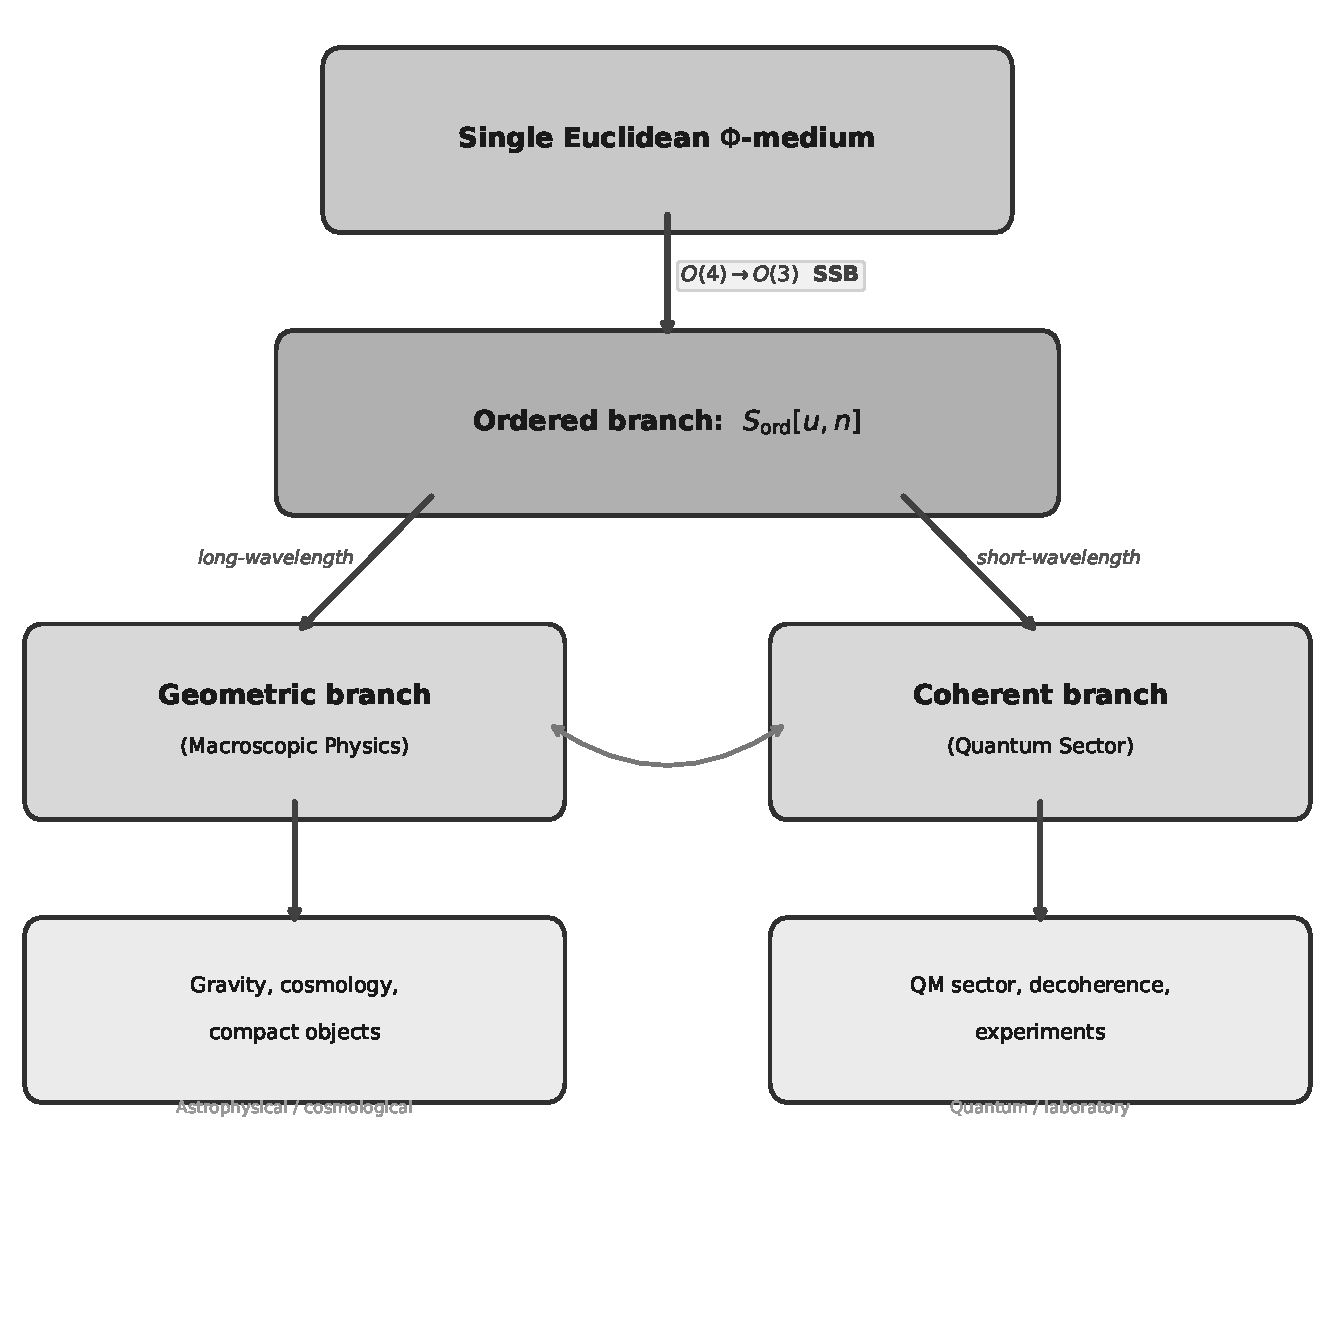
\includegraphics[width=0.88\textwidth]{fig_ect_architecture.pdf}
\caption{Architectural overview of ECT\@. A single Euclidean $\Phi$-field undergoes $O(4) \to O(3)$ symmetry breaking through gradient condensation. Two complementary branches emerge: the geometric branch (gravity, cosmology, galactic dynamics) and the coherent branch (quantum mechanics, decoherence, vacuum effects). All of known physics is organised within this single structure. (\emph{Level~A for the branching architecture; individual arrows carry their own status labels in the preprint.})}
\label{fig:pop_architecture}
\end{figure}

Spontaneous symmetry breaking (SSB) is one of the most powerful organising principles in physics. A spherical magnet has no preferred direction, until it cools below the Curie temperature and all spins align. A perfectly round ball on the tip of a Mexican hat has no preferred position, until it rolls down and selects one valley. In both cases, the underlying laws are symmetric, but the realised state is not.

In ECT, the $\Phi$-medium undergoes an analogous transition: the $O(4)$ symmetry of the four-dimensional Euclidean arena is broken to $O(3)$ (Fig.~\ref{fig:pop_architecture}). Three directions remain equivalent (they become ``space''); one ($w$) is singled out (it becomes the seed of ``time'').

This transition is not merely a technical symmetry breaking. It is the event that makes physics in the familiar sense possible at all. Before ordering, the Euclidean condensate distinguishes no time, no causal order, no preferred class of propagating excitations. After ordering, all of the following arise simultaneously: the causal cone, Lorentzian kinematics, the excitation spectrum, and the decoherence hierarchy. Time is not added to an already prepared physics; it arises together with it as a property of the ordered phase. In this sense the $O(4)\to O(3)$ transition plays the role of a ``crystallisation of the physical world.''

The mechanism behind this transition is \emph{gradient condensation}. In the ordered phase, not the field $\Phi$ itself but its \emph{gradient} $\partial_A\Phi$ acquires a nonzero expectation value pointing in a specific direction: $\langle\partial_A\Phi\rangle = u_0\,\delta_{Aw}$. This distinction is crucial: a nonzero $\langle\Phi\rangle$ would be $O(4)$-invariant (since $\Phi$ is a scalar under rotations, a scalar VEV preserves all rotational symmetries) and would produce no symmetry breaking. The gradient $\partial_A\Phi$, by contrast, transforms as a \emph{vector} under $O(4)$. Its nonzero expectation value breaks the symmetry by selecting a direction --- just as the magnetisation $\langle\mathbf{M}\rangle$ in a ferromagnet is a vector that picks a direction and breaks $O(3) \to O(2)$.

The gradient field can be decomposed into an amplitude and a direction:
\begin{equation}
  \partial_A\Phi = u \cdot n_A,
  \qquad u = |\partial\Phi| \geq 0,
  \qquad n^A n_A = 1.
  \label{eq:pop_polar}
\end{equation}
In the ordered vacuum, $\langle u \rangle = u_0$ and $\langle n^A \rangle = \delta^A{}_w$. This decomposition is the key to the entire theory. Each component plays a distinct physical role:

The \textbf{amplitude mode} ($u$; fluctuations $\sigma = u - u_0$): massive, short-ranged ($\xi_{\rm cond} \sim m_\sigma^{-1} \sim \ell_{\rm Pl}$), connected to gravitational stiffness and the Planck scale. It plays a role analogous to the Higgs boson, but at the Planck scale rather than the electroweak scale.

The \textbf{orientation modes} ($\delta n^A$): three massless Goldstone bosons from $O(4)/O(3) \simeq S^3$. They generate the graviton (spin-2 mode) at the linearised level, plus two additional constrained modes.

The \textbf{phase mode} ($\theta$, in the coherent sector $\Phi_{\rm eff} = \rho\,e^{i\theta}$): connected to gauge fields and quantum dynamics.

The dynamical origin of gradient condensation from the bare action P3 is an open theoretical programme (OP-grad in the preprint). A generalised kinetic action $P(X)$, $X = (\partial_A\Phi)^2$, with a minimum at $X = u_*^2 > 0$, provides the natural dynamical setting for such condensation --- analogous to how a superfluid develops nonzero superflow when the free energy favours a finite condensate velocity. The theory establishes that \emph{given} the ordered branch (P4), a rich and self-consistent effective physics follows.

An important structural result (the ``$P(X)$ no-orientation theorem'', proved in the preprint) shows that a purely kinetic action $P(X)$ can generate gradient condensation (nonzero $u_0$) but \emph{cannot} generate orientation stiffness --- the rigidity that resists bending of the condensate direction. Orientation stiffness must come from higher-order terms or from the NLO sector of the EFT, and it is this stiffness that ultimately gives rise to gravity.


\section{How the Lorentzian signature emerges}
\label{sec:pop_lorentzian}

Once the condensate has selected a direction, the physics of small excitations around the ordered background changes profoundly. The key quantity is the effective kinetic tensor $K^{AB}$ governing fluctuations. The technical preprint proves a uniqueness theorem: the most general quadratic action for fluctuations $\varphi$ around the ordered branch, compatible with the residual $O(3)$ symmetry, takes the form (\emph{Level~A}):
\begin{equation}
  S_{\rm eff} = \int d^4X \left[
  \frac{\beta}{2}(\partial_A\varphi)^2
  - \frac{\alpha}{2}(n^A\partial_A\varphi)^2
  + \ldots\right],
  \label{eq:pop_eft}
\end{equation}
so that
$K^{AB} = \beta\,\delta^{AB} - \alpha\,n^A n^B$.

This tensor has eigenvalues $\beta$ (triply degenerate, along the three directions perpendicular to $n^A$) and $\beta - \alpha$ (along $n^A$). An eigenvalue analysis reveals three distinct regimes:

\emph{If $\alpha < \beta$:} All eigenvalues are positive. The effective metric remains Euclidean. No time, no causal structure, no wave propagation.

\emph{If $\alpha = \beta$:} One eigenvalue vanishes. The system is at the Euclidean--Lorentzian boundary, with degenerate, Galilean-like kinematics.

\emph{If $\alpha > \beta$ (the ``Lorentzian window''):} One eigenvalue is negative. The effective metric acquires a Lorentzian signature $(-,+,+,+)$. Perturbations propagate as waves with a finite speed, and a causal cone structure emerges.

ECT operates in the Lorentzian window. In the canonical benchmark $(\alpha, \beta) = (2, 1)$, the kinetic tensor reduces to $K^{AB} = \delta^{AB} - 2\,n^An^B$, with eigenvalues $(+1, +1, +1, -1)$ --- exactly the Lorentzian signature.

The effective propagation speed is:
\begin{equation}
  c_* = \sqrt{\frac{\beta}{\alpha - \beta}},
  \label{eq:pop_cstar}
\end{equation}
identified with the speed of light (\emph{Level~A/B}).

\textbf{This is the central result of Part~I: the minus sign in the spacetime interval~\eqref{eq:pop_interval} is not assumed but derived.} It appears because the gradient condensate breaks $O(4)$ in a way that produces an anisotropic kinetic tensor with one negative eigenvalue. The derivation status is \emph{Level~A}: it follows from the uniqueness of the kinetic tensor (proved as a theorem) combined with P4.

\textbf{Comparison with other theories.} In Einstein--aether theory (Jacobson, 2004), the anisotropy is introduced by a \emph{postulated} vector field --- not derived from a scalar. In Ho\v{r}ava--Lifshitz gravity, Lorentz invariance is broken \emph{explicitly} at the fundamental level. In Causal Dynamical Triangulations (CDT), the Lorentzian structure is imposed as a constraint on the lattice. In the Hartle--Hawking no-boundary proposal, the Euclidean arena is a computational tool, not a fundamental entity. In ECT alone, the Lorentzian signature is \emph{spontaneously generated} from a higher-symmetry Euclidean substrate, and the result is a theorem, not a phenomenological assumption.

\FloatBarrier

\section{The equation hierarchy: from Euclidean boundary problem to Schr\"odinger}
\label{sec:pop_hierarchy}

\begin{figure}[H]
\centering
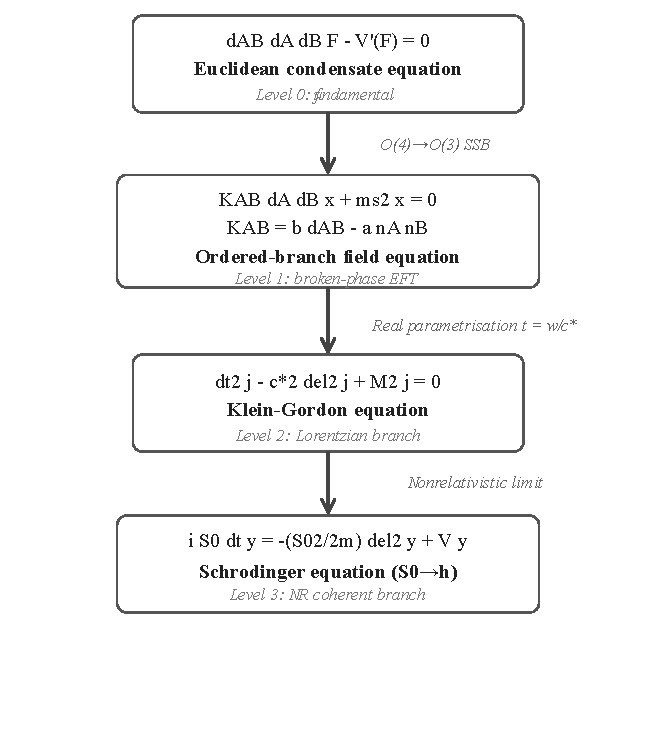
\includegraphics[width=0.55\textwidth]{fig_equation_hierarchy.pdf}
\caption{The ECT equation hierarchy. The fundamental Euclidean field equation (a four-dimensional boundary-value problem) generates the Klein--Gordon equation (after $t = w/c_*$), which in turn yields the Schr\"odinger equation (non-relativistic limit). Each level is a \emph{descendant} of the previous one, not an independent postulate. Standard quantum mechanics occupies the lowest rung. (\emph{Hierarchy structure: Level~A; specific forms: Level~A/B.})}
\label{fig:pop_hierarchy}
\end{figure}

The emergence of Lorentzian signature has a direct consequence for the equations of motion (Fig.~\ref{fig:pop_hierarchy}). The Euclidean field equation $\delta^{AB}\partial_A\partial_B\Phi - V'(\Phi) = 0$ is a four-dimensional \emph{boundary-value problem}: its solutions are determined by data on the \emph{entire boundary} of the Euclidean domain, not by initial data propagated forward in time.

Once the ordered branch is established and we introduce the identification $t = w/c_*$, the same equation, restricted to the Lorentzian window, becomes the \emph{Klein--Gordon equation}: $\partial_t^2\varphi - c_*^2\nabla^2\varphi + m_{\rm eff}^2\varphi = 0$ (\emph{Level~A/B}).

In the non-relativistic limit ($E \approx mc^2 + E_{\rm kin}$, $|E_{\rm kin}| \ll mc^2$), the Klein--Gordon equation reduces to the \emph{Schr\"odinger equation}: $i\hbar\,\partial_t\psi = -\frac{\hbar^2}{2m}\nabla^2\psi + V\psi$ (\emph{Level~A/B}).

This hierarchy is not merely a formal observation. It encodes a physical claim: the Schr\"odinger equation, which standard quantum mechanics takes as its starting axiom, is the \emph{narrowest, lowest-energy descendant} of a more fundamental Euclidean dynamics. The wave equation is \emph{derived}, not postulated.

The distinction between the Cauchy (initial-value) problem of standard QM and the boundary-value problem of ECT is one of the deepest structural differences between the two frameworks. In standard QM, initial data on one time-slice determine the future uniquely. In ECT, the fundamental equation constrains the field configuration on the \emph{entire} four-dimensional domain. This has far-reaching consequences for entanglement, delayed-choice experiments, and the influence of future boundary conditions on present configurations (see Part~III).

\FloatBarrier

\section{Causal cone inheritance and what GW170817 tells us}
\label{sec:pop_cone}

A critical question for any theory claiming to derive Lorentzian spacetime is: why is there a \emph{universal} speed of light? In the real world, photons, gravitons, and all massless particles share the same causal cone to extraordinary precision. A decisive test of any emergent-spacetime framework is whether different low-energy sectors inherit a single causal structure rather than sector-dependent propagation cones---which would destroy universal relativistic kinematics. In ECT the universality of the causal cone is not postulated but inherited from the single ordered condensate background.

In August 2017, the LIGO/Virgo gravitational-wave detectors observed the merger of two neutron stars --- an event designated \textbf{GW170817}. Just 1.7 seconds later (after a journey of 130 million light-years), the Fermi and INTEGRAL satellites detected a gamma-ray burst from the same source. This simultaneous arrival established that the speed of gravitational waves and the speed of light agree to better than one part in $10^{15}$: $|c_{\rm GW}/c - 1| < 6 \times 10^{-15}$.

In many alternative gravity theories (Einstein--aether, Horndeski scalar-tensor models, massive gravity), such universality requires fine-tuning of multiple parameters. In the Standard Model Extension (SME), each particle sector carries an independent set of Lorentz-violation coefficients.

ECT explains this universality as a \emph{structural theorem} (\emph{Level~A/B}). The argument is straightforward:
(i)~The fundamental field is one: $\Phi$.
(ii)~The kinetic tensor is one: $K^{AB}$.
(iii)~All low-energy excitations --- scalar, phase, gauge, tensor --- propagate within the same ordered-branch EFT built on $K^{AB}$.
(iv)~No second independent rank-2 tensor exists in the EFT that could give different sectors different speeds.

The result is \textbf{cross-sector cone universality}:
\begin{equation}
  c_{\rm phase} = c_\gamma = c_{\rm GW} = c_*
  \qquad\text{(\emph{Level~A/B})}.
  \label{eq:pop_cone}
\end{equation}
The GW170817 observation is then not an unexplained coincidence but a \emph{structural consistency check} of ECT. This is one of the theory's most distinctive predictions: the universality of the speed of light is derived from the single-medium origin of all native low-energy sectors.

ECT does admit Planck-suppressed higher-order corrections that can produce tiny sector-dependent speed differences at extreme energies. But arbitrary, unsuppressed, low-energy speed differences between sectors are structurally forbidden. If such differences were ever observed, ECT's one-cone universality would be falsified.


\section{Three fundamental scales from one field}
\label{sec:pop_scales}

\begin{figure}[H]
\centering

\includegraphics[width=0.92\textwidth]{fig_condensate_scales.png}
\caption{The three energy scales of the ECT condensate. A single scalar field generates the Planck/gravitational scale ($\phi_0 \sim 10^{18}$\,GeV), the electroweak scale ($v_2 \sim 246$\,GeV), and the galactic-phenomenology scale ($v_{\rm gal} \sim$ kpc). These are not independent mechanisms but three faces of the same condensate at different organisational levels. (\emph{Level~B for the hierarchy mechanism.})}
\label{fig:pop_scales}
\end{figure}

A notable feature of ECT is that a single scalar field generates three distinct energy scales governing very different regimes of physics (Fig.~\ref{fig:pop_scales}):

The \textbf{gravitational scale} $\phi_0 \sim 2.4 \times 10^{18}$\,GeV (the reduced Planck mass) arises from the symmetry-breaking amplitude of the condensate. It simultaneously determines Newton's constant, Planck's constant, and the speed of light through the matching relations (\emph{Level~B}):
\begin{equation}
  G_N = \frac{c_*^4}{8\pi\phi_0^2}, \qquad
  \hbar = \frac{c_*\phi_0}{\sqrt{\lambda}}, \qquad
  c_* = \sqrt{\frac{\beta}{\alpha-\beta}}.
  \label{eq:pop_matching}
\end{equation}
The fact that a single condensate scale $\phi_0$ simultaneously determines $G$, $\hbar$, and $c$ is a non-trivial structural prediction: these three constants are not independent but are three projections of the same underlying condensate parameter. In standard physics, $c$, $\hbar$, and $G$ appear as three independent empirical constants belonging to different chapters of physics: relativistic kinematics, quantum theory, and gravitation. ECT changes their logical status from external gifts of nature to observable projections of a single underlying medium: $c_*$ expresses the kinematic anisotropy of the ordered phase, $G_N$ expresses the geometric stiffness of the orientation sector, and $\hbar$ expresses the coherent self-consistency of the minimal loop.

The \textbf{electroweak scale} $v_2 \sim 246$\,GeV corresponds to a second, subsidiary condensation within the $\Phi$-sector, generating masses for the $W$, $Z$ bosons, and the Higgs particle. The enormous hierarchy $\phi_0/v_2 \sim 10^{16}$ is addressed through a running-coupling argument: the self-coupling $\lambda$ runs logarithmically with energy and can generate the smaller scale through dimensional transmutation, similar to the mechanism that generates the QCD scale from the running of $\alpha_s$ (\emph{Level~B/Open}).

The \textbf{galactic scale} $r_0 \sim$ kpc marks the transition between Newtonian and modified gravitational behaviour in galaxies, governed by the critical acceleration $g^\dagger \approx cH_0/(2\pi) \approx 1.1 \times 10^{-10}$\,m/s$^2$ (\emph{Level~B}).

Beyond the three primary scales, the same condensate pair $(\phi_0, v_2)$ naturally generates two distinguished intermediate combinations that appear in the neutrino sector: the geometric-mean scale $\sqrt{\phi_0\,v_2} \approx 2.4 \times 10^{10}$\,GeV (close to the scale of thermal leptogenesis and type-I seesaw), and the inverse-ratio Weinberg-operator scale $v_2^2/\phi_0 \approx 2.5 \times 10^{-5}$\,eV (within a few orders of magnitude of the observed neutrino mass splittings). Both combinations are the two simplest dimensionally consistent products that can be built from the same pair of fundamental ECT parameters; their joint appearance in the neutrino sector is a structural consequence of the three-scale hierarchy rather than an independent numerical coincidence. This further illustrates how the condensate architecture organises multiple observed energy scales from a single underlying medium (\emph{Level~B/C}).

\FloatBarrier

\section{ECT loops, quantisation, and the origin of $\hbar$}
\label{sec:pop_loops}

A distinctive feature of ECT is how quantisation emerges naturally from the compact-phase structure of the condensate, without being imposed as an axiom.

In the coherent sector, the effective order parameter has the polar form $\Phi_{\rm eff} = \rho\,e^{i\theta}$, where $\theta$ is a compact (periodic) phase variable. The single-valuedness requirement (BR1) means that if we transport $\theta$ around any closed loop $\mathcal{C}$ in the Euclidean manifold, it must return to its original value:
\begin{equation}
  \oint_{\mathcal{C}} \partial_A\theta\,dX^A = 2\pi n,
  \qquad n \in \mathbb{Z}.
  \label{eq:pop_winding}
\end{equation}
This is not a quantum axiom --- it is a \emph{topological necessity} for any smooth, single-valued function with compact range.

The consequence is immediate: the action associated with loop configurations is quantised. The minimal nontrivial loop ($n = 1$) carries a definite action:
\begin{equation}
  S_{\rm loop,min} = 2\pi S_0,
  \label{eq:pop_Sloop}
\end{equation}
where the scale $S_0$ depends on the condensate parameters. Through the matching relation~\eqref{eq:pop_matching}, $S_0$ is identified with $\hbar$ (\emph{Level~B}).

This means Planck's constant is not a mysterious fundamental quantity in ECT. It is the action scale set by the condensate's compact-phase structure --- just as the flux quantum $\Phi_0 = h/(2e)$ in a superconductor is set by the Cooper pair condensate, and the Bohr--Sommerfeld condition $\oint p\,dq = nh$ is set by the periodicity of classical action variables. All three are instances of the same mathematical mechanism: \emph{single-valuedness of a periodic order parameter implies quantisation}.

The loop sectors partition the coherent branch into topologically distinct classes indexed by the integer $n$. Configurations in different sectors cannot be continuously deformed into each other. This is why quantum interference can arise in ECT without operator axioms: paths belonging to different winding sectors contribute to the path sum with different phase factors, producing constructive or destructive combination.


\section{The arrow of time, the second law, and why time flows}
\label{sec:pop_arrow}

In the Euclidean picture, the coordinate $w$ is just one of four equivalent spatial directions. There is no ``forward'' or ``backward'' in $w$, just as there is no ``forward'' in $x$. The arrow of time is not fundamental: it is \emph{emergent}.

ECT constructs the thermodynamic arrow in two stages:

\textbf{Stage 1: directional backbone (\emph{Level~A}).} In the Lorentzian branch, the effective dynamics admits a retarded causal structure: perturbations propagate forward along $w$ inside the emergent light cone. The dissipative kernel of the influence-functional formalism is positive-semidefinite ($\Gamma_{\rm irr} \geq 0$), meaning that off-diagonal histories are \emph{suppressed} rather than amplified. This gives the \emph{directionality} of decoherence.

\textbf{Stage 2: entropy growth (\emph{Level~B}).} Under two additional effective-closure assumptions --- an ohmic spectral density and a Markovian regime --- the coarse-grained entropy satisfies:
\begin{equation}
  \frac{dS_{\rm ent}}{dw} = N_{\rm eff}\,\gamma
  \left(\frac{dq}{dw}\right)^2 \geq 0,
  \label{eq:pop_2ndlaw}
\end{equation}
where $N_{\rm eff}$ is the effective number of environmental modes and $\gamma$ is the decoherence rate per mode. The sign is anchored in the Level~A retarded structure; the explicit formula requires Level~B closure.

The result is a three-regime picture:

At the \emph{cosmological} level, the ordered branch defines the cosmic arrow; the second law holds to overwhelming accuracy.

At the \emph{macroscopic} level ($N_{\rm eff} \gg 1$), the ratio of backward-to-forward transition probabilities is exponentially suppressed: $P_{\rm back}/P_{\rm fwd} = \exp(-2N_{\rm eff}\gamma\,\Delta w \cdot (\Delta q)^2/\ell^2)$. For a mole of gas at room temperature over a nanosecond, the exponent is $\sim 3.6 \times 10^{33}$ --- reverse trajectories are fantastically unlikely.

At the \emph{quantum} level ($N_{\rm eff} \sim 1$), the exponent becomes tiny ($\sim 10^{-15}$), and effective time-reversibility is recovered --- consistent with the well-known fact that isolated quantum systems evolve reversibly.

The second law is therefore not an independent postulate in ECT. Its directional backbone is Level~A; its full monotonicity is Level~B. What ECT adds beyond Boltzmann is a \emph{structural explanation} of why the initial condition is special: it is tied to ordered-branch selection (P4), not imposed ad hoc.


\section{Spectrum, branching, gauge symmetries, and particles}
\label{sec:pop_spectrum_etc}

\begin{figure}[H]
\centering
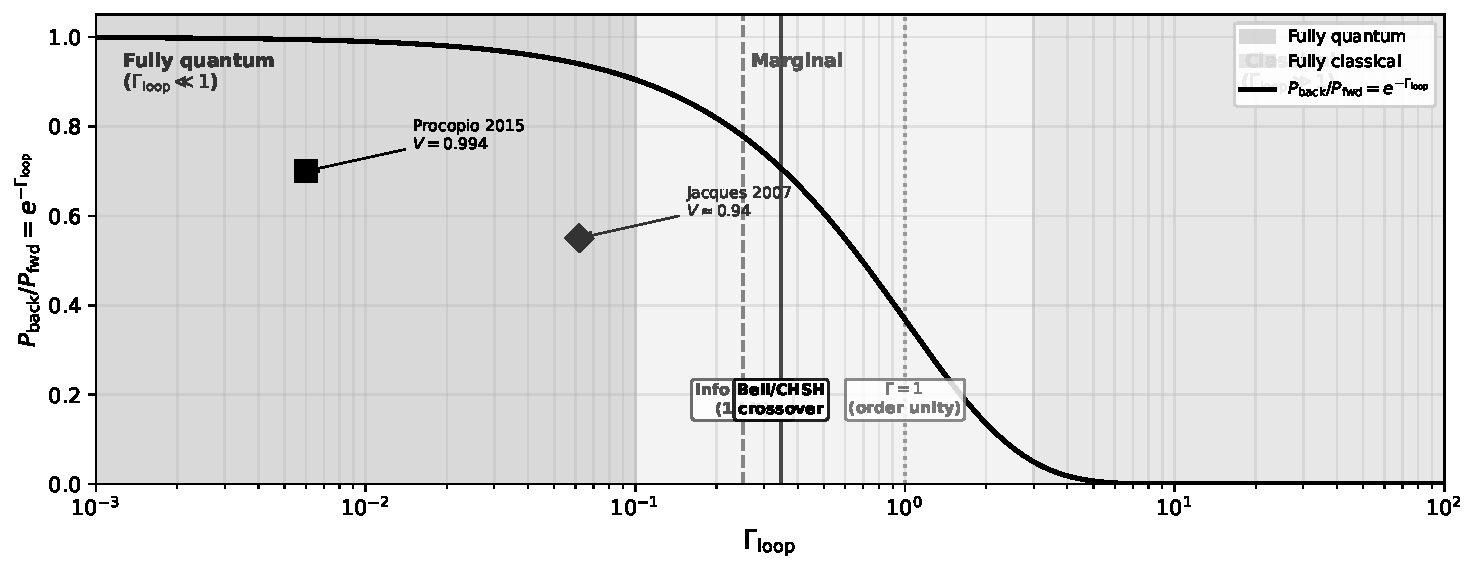
\includegraphics[width=0.88\textwidth]{fig_gamma_crossover.pdf}
\caption{The quantum--classical boundary. The dimensionless decoherence parameter $\Gamma_{\rm loop}$ determines whether a system behaves quantum-mechanically ($\Gamma_{\rm loop} \ll 1$) or classically ($\Gamma_{\rm loop} \gg 1$). The crossover at $\Gamma_{\rm loop} \sim 1$ defines the quantum--classical boundary. Different objects --- electron, C$_{60}$, bacterium, dust grain, cat --- occupy different positions on this scale. (\emph{Level~A for the crossover structure; Level~B for numerical estimates.})}
\label{fig:pop_gamma}
\end{figure}

The ordered condensate supports three classes of excitations, each playing a distinct physical role:

\textbf{Amplitude mode ($\sigma$):} Fluctuations of the gradient magnitude $u$ around $u_0$. This mode is massive ($m_\sigma^2 = 2\mu^2$, \emph{Level~A}), with correlation length $\xi_{\rm cond} \sim m_\sigma^{-1}$ identified with the Planck length (\emph{Level~B}). It is heavy, short-ranged, and plays a role analogous to the radial Higgs mode at the Planck scale.

\textbf{Orientation modes ($\delta n^A$):} The symmetry breaking $O(4)/O(3)$ naively suggests three Goldstone bosons; however, the integrability constraint on the scalar-only ECT basis reduces the physically independent propagating soft content to a single surviving longitudinal scalar mode $\chi$ (massless at tree level). Their dynamics generates the graviton (spin-2, massless) at the linearised level (\emph{Level~A}), plus constrained scalar/vector companions. An important structural point is that the amplitude mode is too heavy ($m_\sigma \sim M_{\rm Pl}$) for kpc-scale variations, ruling out naive scalar-field dark matter models --- a powerful constraint that uniquely selects the viable mechanism for galactic phenomenology (Part~II).

\textbf{Phase mode ($\theta$):} In the coherent sector, phase fluctuations connect to gauge fields: the photon emerges as the gauge boson of the $U(1)$ phase symmetry (\emph{Level~A/B after P5}).

The ordered condensate organises into two complementary branches (Fig.~\ref{fig:pop_gamma}): the \textbf{geometric branch} (Macroscopic Physics, long-wavelength, coarse-grained, $\Gamma_{\rm loop} \gg 1$) and the \textbf{coherent branch} (Quantum Sector, short-wavelength, phase-coherent, $\Gamma_{\rm loop} \ll 1$). Both originate from the same ordered condensate action $S_{\rm ord}[u, n]$ (\emph{Level~A}). The quantum--classical boundary corresponds to the crossover $\Gamma_{\rm loop} \sim 1$.

\subsection{Gauge symmetries and the four fundamental interactions}
\label{sec:pop_gauge}

ECT does not postulate gauge symmetries. It derives them from the internal structure of the $\Phi$-medium through P5. Since pointwise values of $\theta$ and $n_A$ are not observable, local redefinitions must leave physics unchanged --- requiring compensating gauge connections.

\textbf{Electromagnetism (\emph{Level~A/B after P5}):} The compact phase $\theta$ generates a $U(1)$ gauge symmetry. Local phase rotations require a gauge field $A_\mu$ satisfying Maxwell's equations. The photon is the gauge boson of this emergent symmetry.

\textbf{Weak interaction (\emph{Level~B}):} The $O(3)$ residual symmetry provides a natural $SU(2)$ structure. Combined with electroweak condensation at $v_2 \sim 246$\,GeV: $W^\pm$, $Z$ bosons and electroweak symmetry breaking.

\textbf{Strong interaction (\emph{Level~B/Open}):} A structural route to $SU(3)$ colour is proposed through a minimal colour completion: exact colour requires a separate internal complex rank-3 module with $SU(3)$-structure (Hermitian metric + complex volume form), independent of the singlet condensate. A deeper geometric candidate ($G_2$ internal structure) is also identified. Full QCD derivation remains open.

\textbf{Gravity (\emph{Level~A/B}):} Gravity arises from orientation stiffness --- the condensate's resistance to bending of $n^A$ (Part~II).

Thus all four fundamental interactions have a common condensate origin. Beyond these four, ECT predicts a \textbf{fifth, Planck-suppressed fermion--condensate coupling} (\emph{Level~B}): a spin-precession frequency $\omega_5 \sim 10^{-10}$\,rad/s and an E\"otv\"os parameter $\eta \sim 10^{-15}$, testable by MICROSCOPE-2.

\subsection{Elementary particles}

The particle spectrum includes the graviton (spin-2 from $\delta n^A$, \emph{Level~A}), photon ($U(1)$, \emph{Level~A/B}), $W^\pm$/$Z$ ($SU(2)$, \emph{Level~B}), Higgs (electroweak radial mode, \emph{Level~B}), gluons ($SU(3)$, \emph{Level~B/Open}), fermions ($O(3)$ spinors with Dirac equation reconstructed via vierbein formalism, \emph{Level~A/B}), and instantons ($m_n = n \times 1.6$\,GeV/$c^2$, \emph{Level~B}).

What remains open (\emph{Level~Open}): the origin of three fermion generations; the Yukawa coupling hierarchy; the fine-structure constant $\alpha = 1/137$. Qualitative structural routes exist (e.g.\ generations may be related to topological sectors of $S^3$), but rigorous quantitative derivations do not.

\textbf{Three logical classes of excitations.}
ECT does not place all particles on the same logical footing---a fundamental difference from standard QFT.
Category~(i), the \emph{required condensate excitations} (graviton, radial mode $\sigma$, soft mode $\chi$), are analogous to phonons in a crystal: they are inevitable consequences of an ordered medium with broken symmetry.
Category~(ii), the \emph{structurally embedded Standard Model fields} (photon, $W^\pm$, $Z$, Higgs, fermions, gluons), are analogous to impurity atoms in a lattice: compatible with the medium but not derived from the minimal scalar action.
Category~(iii), the \emph{topological sectors} (textures from $\pi_3(S^3)=\mathbb{Z}$; anti-predictions from $\pi_0=\pi_1=\pi_2=0$: no monopoles, no domain walls, no cosmic strings), are analogous to dislocations: determined by the topology of the vacuum manifold.
In standard QFT all fields are equally fundamental postulates; in ECT they occupy different logical tiers.

\textbf{Multi-particle description and the status of Fock space.}
Ordinary quantum mechanics works with a fixed number of particles~$N$. Processes with variable~$N$ (emission, annihilation, pair creation) require quantum field theory, where the Fock space and creation/annihilation operators are additional postulates. In ECT, changing particle number is a reconfiguration of one condensate medium---analogous to vortices appearing and disappearing in a superfluid. ECT does not require Fock space as a fundamental postulate; however, an explicit emergent sector decomposition with variable excitation number remains to be constructed from condensate dynamics (Open; OP-Q11). This is a nontrivial reconstruction problem, not a foundational gap.

Multi-particle description is necessary even in the coherent branch (where no event-like Lorentzian interaction is available) for four reasons: (a)~entanglement as non-factorisable common-medium correlation; (b)~exchange statistics ($\pi_1(\mathcal{M}_2)=\mathbb{Z}_2$); (c)~the decoherence threshold, which depends on $N_{\rm eff}$; (d)~processes with variable excitation number.

Figure~\ref{fig:pop_partI_logic} summarises the derivation logic of Part~I.


\section{Conclusions of Part~I}

\subsection{Principal results}

From six postulates (P1--P6) and one derived branch rule (BR1), the following structures are obtained:

\begin{enumerate}
\item Lorentzian signature $(-,+,+,+)$ from $O(4)\to O(3)$ SSB (\emph{A}).
\item Universal causal cone: all species share $c_*=c$ (\emph{A/B}).
\item Equation hierarchy: Euclidean $\to$ KG $\to$ Schr\"odinger (\emph{A/B}).
\item Arrow of time from monotonic decoherence (\emph{A}).
\item Second law: $dS_{\rm ent}/dw \geq 0$ (\emph{A/B}).
\item Branching into geometric and coherent sectors (\emph{A}).
\item $U(1)$ electromagnetism from P5 (\emph{A/B}).
\item $SU(2)$ weak sector (\emph{B}); $SU(3)$ colour (\emph{B/Open}).
\item Graviton as spin-2 orientation mode (\emph{A}).
\item $S_0 = \hbar$ from compact-phase winding (\emph{B}).
\item Quantisation from loop-sector topology (\emph{A}).
\item Fifth-force coupling $\beta_5 \sim m_f/\bar{M}_{\rm Pl}$ (\emph{B}).
\end{enumerate}

\subsection{Key equations and principles of Part~I}

Effective kinetic tensor: $K^{AB} = \beta\,\delta^{AB} - \alpha\,n^An^B$ (uniqueness theorem).

Propagation speed: $c_* = \sqrt{\beta/(\alpha-\beta)}$.

Matching relations: $G_N = c_*^4/(8\pi\phi_0^2)$, $\hbar = c_*\phi_0/\sqrt{\lambda}$.

Loop quantisation: $\oint \partial_A\theta\,dX^A = 2\pi n$; $S_{\rm loop,min} = 2\pi\hbar$.

Cross-sector universality: $c_{\rm phase} = c_\gamma = c_{\rm GW} = c_*$.

Second law: $dS_{\rm ent}/dw = N_{\rm eff}\gamma(dq/dw)^2 \geq 0$.

\subsection{Predictions originating in Part~I}

GW170817 consistency: $|c_{\rm GW}/c - 1| < 6\times10^{-15}$ (satisfied).

Fifth force: $\omega_5 \sim 10^{-10}$\,rad/s, $\eta \sim 10^{-15}$ (MICROSCOPE-2).

LIV: $\Delta t_{\rm GW} \sim 10^{-64}$\,s (Planck-suppressed, currently unobservable).

Casimir boundary-sensitive vacuum response (conditional; soft-mode counting provisional).

\subsection{Part~I derivation logic}

\begin{figure}[H]
\centering

\includegraphics[width=\textwidth]{fig_partI_derivation_logic_pop.pdf}
\caption{Part~I derivation logic. From six postulates and BR1, the theory derives: Lorentzian signature, universal causal cone, equation hierarchy, arrow of time, second law, branching, gauge symmetries, particles, quantisation. Colours indicate Level~A, B, and Open status.}
\label{fig:pop_partI_logic}
\end{figure}

Figure~\ref{fig:pop_partI_logic} shows the complete derivation architecture of Part~I.

\FloatBarrier

\newpage
%==============================================================
\part{Macroscopic Physics: Gravity, Cosmology, and Observational Tests}
\label{part:macro_pop}
%==============================================================

\section{Special Relativity as the homogeneous limit}

In the homogeneous ordered phase, where the condensate amplitude and direction are uniform throughout space, the effective metric reduces to the Minkowski form: $ds^2 = -c_*^2 dt^2 + dx^2 + dy^2 + dz^2$. All familiar consequences of special relativity follow as theorems: Lorentz transformations arise as the invariance group of the causal cone; time dilation and length contraction are kinematic consequences; $E^2 = p^2c^2 + m^2c^4$ follows from the effective wave equation. In ECT, special relativity is a \emph{derived limit} (\emph{Level~A}), not an independent postulate.

\subsection{The universal speed bound}

One of the most familiar facts of physics --- that nothing can travel faster than light --- is, in standard special relativity, a direct consequence of Einstein's second postulate. In ECT, this fact is not postulated: it is a theorem.

The argument rests not on any particular type of excitation but on the \emph{characteristic cone} of the ordered-branch field equation. The principal symbol of the equation of motion for~$\Phi$ defines a unique causal cone with speed~$c_*$. Through the symmetric-hyperbolic structure of the dynamics and the Leray--Choquet-Bruhat theorem, ECT establishes at Level~A that the domain of dependence of any point lies strictly inside its past causal cone, and that no ordered-branch disturbance --- linear or nonlinear --- propagates outside the cone. This is a theorem about the full nonlinear scalar dynamics, not merely about linearised waves.

For linear plane waves, the bound takes a concrete form. A massive mode has a group velocity strictly less than~$c_*$, with equality only in the massless limit: massive excitations travel inside the cone, massless excitations on its boundary.

An important subtlety deserves mention. The \emph{phase velocity} of massive modes formally \emph{exceeds}~$c_*$. This is a well-known feature of relativistic wave equations and is \emph{not} a violation of causality: phase velocity does not carry information. The causal bound is set by the characteristic cone --- the front speed --- not by the phase velocity. This distinction highlights the correct ECT formulation: the speed limit is a bound on \emph{causal propagation}, not on every quantity one can label a ``velocity''.

\subsection{Signal speed, not photon speed}

A deeper point emerges from the ECT derivation. The fundamental limiting velocity is not ``the speed of light'' as a photon-specific constant. It is the \emph{signal speed} of the ordered-branch causal cone --- the maximum speed of causal influence, front propagation, and information transfer.

The photon merely \emph{realises} this boundary speed. It does so because the emergent Abelian gauge boson is massless (the relevant $U(1)$ symmetry remains unbroken, and gauge invariance forbids a mass term) and because the gauge sector inherits the same causal cone as the scalar branch. Gravitational waves likewise inherit the same cone in the minimal tensor route. The near-equality confirmed by GW170817 ($|c_{\rm GW}/c - 1| < 6 \times 10^{-15}$) is therefore a structural consistency check, not a coincidence.

Because inertial coordinate changes in the homogeneous ordered branch are precisely the transformations preserving one and the same null cone, the same vacuum signal speed is measured in every inertial frame. What Einstein postulated as the universality of the vacuum light speed is, in ECT, reduced to a structural consequence of the unique ordered-branch causal cone (\emph{Level~A}) together with cone inheritance in the minimal gauge route (\emph{Level~A/B}).

In this sense, the vacuum speed of light is not fundamental by itself; it is the experimentally accessible manifestation of the deeper ordered-branch causal speed.


\section{Emergent gravity and the generalised Einstein equations}
\label{sec:pop_gravity}

In ECT geometry is not the primitive ontology. The effective metric is a derived bookkeeping object encoding how excitations propagate on the ordered condensate background. Gravity is not a fundamental force but the long-wavelength geometric response of the ordered condensate to deformations of its orientation structure~$n^A$. The graviton is not a quantum of fundamental geometry but a low-energy excitation of the condensate order. This inverts the conventional logic of quantum gravity: ECT replaces the question ``how to quantise an existing geometry?'' with the question ``how do collective condensate excitations produce a geometric description?''.

The mechanism is analogous to elastic stresses in a crystal lattice. When matter bends $n^A$ away from equilibrium, ``orientation stress'' acts as an effective gravitational field.

The derivation proceeds through stages. The orientation stiffness $\kappa_n \sim u_0^2/m_\sigma^2 \sim \phi_0^2$ determines the energy cost of bending $n^A$. Linearising around the flat background, transverse-traceless fluctuations satisfy a spin-2 wave equation identical to linearised GR (\emph{Level~A/B}).

At the nonlinear level, ECT derives \textbf{generalised Einstein equations (GEE)}:
\begin{equation}
  G_{\mu\nu} + \Lambda_{\rm eff}\,g_{\mu\nu}
  = 8\pi G_{\rm eff}\,T_{\mu\nu} + \Theta_{\mu\nu}[n],
  \label{eq:pop_gee}
\end{equation}
where $\Theta_{\mu\nu}[n]$ is the orientation-stress tensor (\emph{Level~B}). This term has no analogue in standard GR. It vanishes in homogeneous configurations but becomes dynamically important in three distinct observational domains:

On \emph{galactic scales}, $\Theta_{\mu\nu}$ provides the additional acceleration that explains flat rotation curves without particle dark matter (Section~\ref{sec:pop_galaxies}).

On \emph{cluster scales}, it modifies gravitational lensing morphology, reproducing the Bullet Cluster offset without dark matter halos (Section~\ref{sec:pop_clusters}).

In \emph{cosmology}, the evolving $G_{\rm eff}$ and $\Theta_{\mu\nu}$ jointly address the Hubble tension and the JWST problem (Sections~\ref{sec:pop_hubble}--\ref{sec:pop_jwst}).

Gravitational waves propagate at $c_*$ with two transverse-traceless modes (\emph{Level~A/B}), consistent with LIGO/Virgo. Weak-field and post-Newtonian limits reproduce Newtonian gravity and are compatible with Solar System tests (PPN parameters).


\section{Condensate evolution and cosmic history}
\label{sec:pop_evolution}

\begin{figure}[H]
\centering

\includegraphics[width=\textwidth]{ect_vs_lcdm_comparative_timeline_bw.pdf}
\caption{Cosmic timeline comparison: $\Lambda$CDM (top) and ECT (bottom). The earliest epoch in ECT is a timeless Euclidean phase; the transition $O(4) \to O(3)$ creates time itself. The lower panel shows the condensate amplitude $u_0(t)$, scale factor $a(t)$, and effective gravitational coupling $G_{\rm eff}(t)$. (\emph{Level~A for the pre-Lorentzian regime; Level~B for the detailed timeline.})}
\label{fig:pop_timeline}
\end{figure}

In $\Lambda$CDM, the universe begins at $t=0$ (the Big Bang singularity) and proceeds through inflation, nucleosynthesis, recombination, structure formation, and dark-energy domination. ECT tells a fundamentally different story (Fig.~\ref{fig:pop_timeline}).

Before the $O(4) \to O(3)$ transition, there is no time at all. The universe exists as a four-dimensional Euclidean medium with full $O(4)$ symmetry. The concept of ``before'' has no meaning in the usual temporal sense. The Big Bang singularity is replaced by the ordering transition, at which the condensate amplitude $u_0$ grows from zero to its equilibrium value $\phi_0 \sim \bar{M}_{\rm Pl}$. This growth naturally produces a period of rapid ordered-branch expansion, replacing the standard inflationary postulate with a pre-Lorentzian Euclidean ordering picture.

After the ordering is established, the evolution shares familiar milestones (nucleosynthesis, recombination, galaxy formation), but two features distinguish ECT from $\Lambda$CDM: the gravitational coupling $G_{\rm eff}$ evolves slowly with redshift, and the dark-energy component arises from residual condensate energy rather than from a cosmological constant.

A notable consequence is the \textbf{age of the Lorentzian branch}. In ECT, ``the age of the universe'' refers to the duration of the ordered Lorentzian branch, not the time since a fundamental singularity. Because $G_{\rm eff}(z) > G_N$ at high redshift, the Hubble rate $H(z)$ is larger over part of cosmic history, which reduces the age integral $t_0 = \int_0^\infty dz/[(1+z)H(z)]$. Benchmark estimates give $t_0^{\rm ECT} \approx 13.0$--$13.5$\,Gyr, modestly shorter than the $\Lambda$CDM value of $\sim 13.8$\,Gyr (\emph{Level~B}). This reduction arises directly from the enhanced early-time gravity and is not a separate assumption. It has consequences for the JWST problem discussed below.

At late times, ECT admits two scenarios: Scenario~A ($u_0 \to \text{const}$, eternal expansion) and Scenario~B ($u_0 \to 0$, recollapse on a timescale $\sim 10^{100}$\,years). Distinguishing these requires data not yet available.


\section{The four classical cosmological problems}
\label{sec:pop_cosmo_problems}

The standard Big Bang model faces four well-known puzzles. The conventional resolution invokes cosmic inflation --- a brief period of exponential expansion driven by a hypothetical inflaton field. While inflation is remarkably effective, it introduces its own unresolved issues: the inflaton has never been directly observed; inflation requires specific initial conditions to start (the initial homogeneity problem --- inflation itself needs a sufficiently uniform region to begin, yet it was introduced to \emph{explain} homogeneity); the measure problem makes probabilistic predictions ill-defined in the context of eternal inflation; and the trans-Planckian problem arises because CMB modes observed today had sub-Planckian wavelengths at the onset of inflation, potentially probing unknown physics.

ECT resolves all four puzzles at the level of the ordering transition itself, without introducing an inflaton field and without encountering any of these difficulties.

\subsection{The horizon problem}

The cosmic microwave background (CMB) --- relic radiation from 380\,000 years after the Big Bang --- is uniform to one part in $10^5$ across the entire sky. In $\Lambda$CDM, opposite sides of the sky were never in causal contact at that epoch: their past light cones do not overlap. The uniformity is unexplained without inflation.

In ECT, the resolution is structural (\emph{Level~A for the pre-ordered regime; Level~B for its cosmological realisation}). Before the $O(4) \to O(3)$ transition, the Euclidean phase has no causal structure at all: there are no light cones, no causal horizons, no ``regions out of contact.'' All points of $\mathcal{M}^4$ are connected by the Euclidean metric. Uniformity across the CMB is inherited from the symmetric pre-Lorentzian phase.

\subsection{The flatness problem}

Observations show $|\Omega_k| < 0.002$ (Planck 2018). In $\Lambda$CDM, this requires fine-tuning to $\sim 10^{-60}$.

In ECT: the Euclidean manifold $\mathcal{M}^4$ in P1 is flat by construction ($\delta_{AB}$). Spatial flatness of the emergent Lorentzian geometry is a structural consequence of the flat substrate (\emph{Level~A}).

\subsection{The relic and monopole problem}

Grand Unified Theories predict massive topological defects (magnetic monopoles). None observed. In ECT: the vacuum manifold $S^3$ has $\pi_2(S^3) = 0$ --- \emph{no stable monopoles are topologically possible} (\emph{Level~A}).

\subsection{The primordial perturbation problem}

The CMB contains tiny fluctuations ($\sim 10^{-5}$) with a nearly scale-invariant spectrum ($n_s = 0.9649 \pm 0.0042$, Planck 2018). In ECT, the ordered branch carries exactly one independent scalar perturbation mode at leading order (\emph{Level~A}). Plausible condensate-evolution scenarios produce $n_s \sim 0.967$ for 60 e-folds, consistent with observations. The full first-principles derivation of $n_s$, $r$, and $A_s$ remains \emph{Level~B/Open}.

\subsection{Summary}

All four problems are resolved without introducing an inflaton field, without fine-tuning initial conditions, and without the measure, trans-Planckian, and initial-homogeneity difficulties that inflation carries. The pre-Lorentzian Euclidean phase provides a natural starting point from which the Lorentzian ordered branch inherits uniformity, flatness, topological simplicity, and a single-mode perturbation sector. Phenomenological introduction of inflation is unnecessary.


\section{The dark sector in ECT}
\label{sec:pop_dark}

The terms ``dark matter'' and ``dark energy'' were introduced phenomenologically to account for observations that standard gravity with visible matter alone cannot explain: flat rotation curves, gravitational lensing, large-scale structure, accelerated expansion. These phenomena are real and well-established. However, the entities postulated to explain them --- invisible particles (WIMPs, axions, sterile neutrinos) and a cosmological constant $\Lambda$ --- have never been directly confirmed despite decades of dedicated searches. ECT provides a unified structural explanation for the entire dark sector from the condensate dynamics, without introducing any new fundamental entities.

\subsection{Dark matter: condensate response, not particles}

In $\Lambda$CDM, the flat rotation curves of galaxies, gravitational lensing in clusters, and the large-scale structure of the universe are attributed to an invisible component --- dark matter particles --- constituting $\sim 27\%$ of the energy budget. Despite extensive experimental programmes spanning direct detection (LUX, XENON, PandaX, LZ), indirect detection (Fermi-LAT, AMS-02), and collider searches (LHC), no dark matter particle has ever been observed. The parameter space for WIMPs --- once the leading candidate --- is almost entirely excluded.

In ECT, all observational phenomena attributed to dark matter arise from the nonlinear response of the condensate amplitude $\phi$ in weak gravitational fields (\emph{Level~B}). The orientation-stress tensor $\Theta_{\mu\nu}[n]$ in the generalised Einstein equations~\eqref{eq:pop_gee} provides additional effective gravitational acceleration in the regimes where dark matter is conventionally invoked: galaxy outskirts, cluster environments, and cosmological scales. Flat rotation curves, the BTFR, the RAR, and cluster lensing offsets are all reproduced without a single dark matter particle (Sections~\ref{sec:pop_galaxies}--\ref{sec:pop_clusters}).

\subsection{Dark energy: condensate residual energy, not a cosmological constant}

In $\Lambda$CDM, the accelerated expansion of the universe is attributed to a cosmological constant $\Lambda$ --- a fixed parameter responsible for $\sim 68\%$ of the total energy budget. No fundamental theory explains its value, which differs from quantum field theory estimates by approximately 120 orders of magnitude (the cosmological constant problem).

In ECT, what appears as dark energy is the \emph{residual amplitude energy} of the ordered condensate background --- the same medium that produces gravity and quantum mechanics. No independent cosmological constant or dark-energy substance is postulated. The equation-of-state parameter satisfies $w_0 \neq -1$, unlike the fixed $w = -1$ of a cosmological constant; ECT predicts $w_0 \approx -0.83$, compatible with DESI 2024 results which found evidence for dynamical dark energy at $\sim 2.5\sigma$ significance. If $w = -1$ is confirmed with high precision by future surveys (DESI, Euclid), the ECT late-time acceleration closure would be falsified. Conversely, if dynamical dark energy is confirmed, ECT provides a structural explanation while $\Lambda$CDM does not.

A structural advantage of the ECT reframing: loop contributions to the vacuum energy are finite (the physical cutoff is $m_\sigma\sim M_{\rm Pl}$, not infinity), and the effective cosmological contribution is a dynamical functional of the condensate background rather than a rigid constant. This does not yet solve the 120-orders-of-magnitude fine-tuning problem; it reframes it as a question about condensate dynamics rather than a divergent sum over zero-point energies (\emph{Open: OP-$\Lambda$3}).

\subsection{ECT reinterpretation of the dark sector}

Within the minimal ECT benchmark developed here, the phenomena usually attributed to dark matter particles and to a cosmological constant are reinterpreted as condensate-response effects: condensate-induced gravitational response for galactic mass-discrepancy phenomenology, and ordered-branch background dynamics for late-time accelerated expansion. The terms ``dark matter'' and ``dark energy'' are retained as labels for observational phenomena for comparison with the literature; they do not refer to independent physical substances in ECT. The present benchmark does not require dark matter particles or an independent cosmological constant to account for the observational data. This does not yet exclude every possible ECT extension with additional weakly coupled condensate excitations; it states only that the present minimal framework does not need them.

\textbf{Important interpretive caveat.} The statement ``ECT does not need dark matter particles in its minimal benchmark'' is not equivalent to ``ECT proves that no particle beyond the Standard Model can ever exist.'' The first is a statement about the present minimal closure. The second would be an overclaim that the theory does not make. Collective condensate excitations and topological sectors remain structurally possible as optional extensions; they are not required by the core benchmark fit.


\section{The Hubble tension}
\label{sec:pop_hubble}

\begin{figure}[H]
\centering

\includegraphics[width=0.82\textwidth]{ect_h0_scan_bw.pdf}
\caption{The ECT Hubble-tension alleviation mechanism. The evolving effective gravitational coupling $G_{\rm eff}(z) > G_N$ at high redshift shifts the inferred Hubble constant upward by $\sim 3$\,km/s/Mpc. (\emph{Sign: Level~A structural prediction; magnitude: Level~B.})}
\label{fig:pop_hubble}
\end{figure}

The Hubble constant $H_0$ measures the current expansion rate of the universe. Two independent methods give discrepant results: the Planck satellite, analysing the CMB assuming $\Lambda$CDM, infers $H_0 = 67.4 \pm 0.5$\,km/s/Mpc; the SH0ES team, using the cosmic distance ladder (Cepheids + Type~Ia supernovae), measures $H_0 = 73.0 \pm 1.0$\,km/s/Mpc. The discrepancy exceeds $5\sigma$ and is known as the \emph{Hubble tension} --- one of the most pressing open problems in cosmology.

ECT offers a structural alleviation mechanism (Fig.~\ref{fig:pop_hubble}). At high redshift, the condensate was slightly less screened, meaning $G_{\rm eff}(z) > G_N$. Specifically, $G_{\rm eff}(z) \approx G_N(1+z)^{2\varepsilon}$ with $\varepsilon \approx 0.01$. The enhanced gravity reduces the angular diameter distance to the last scattering surface; a CMB-calibrated analysis then interprets this as a higher $H_0$, shifted upward by $\sim 3$\,km/s/Mpc --- the direction and approximate magnitude needed.

The \emph{sign} of the shift is a structural prediction (\emph{Level~A}): any ordered-branch background with $G_{\rm eff} > G_N$ at high~$z$ necessarily shifts $H_0$ upward. The magnitude is closure-dependent (\emph{Level~B}). The same condensate background simultaneously affects the age budget and early structure formation, producing correlated predictions rather than independent parameters.


\section{The JWST early-galaxy problem}
\label{sec:pop_jwst}

The James Webb Space Telescope (JWST), launched in December 2021, has detected galaxies at redshifts $z > 10$, when the universe was less than 500 million years old. Several are unexpectedly massive and mature --- containing old stellar populations, organised disk structures, and chemical enrichment that seem to require more formation time than $\Lambda$CDM allows. Standard structure formation with fixed $G_N$ cannot produce such objects quickly enough.

ECT addresses this through two complementary mechanisms, both arising from the same ordered-branch condensate dynamics:

First, the evolving $G_{\rm eff}(z) > G_N$ at high~$z$ means gravitational collapse was \emph{more efficient} in the early universe.

Second, the GEE~\eqref{eq:pop_gee} include $\Theta_{\mu\nu}[n]$, which provides additional effective attraction beyond a simple scalar-tensor model.

It is important to note that the shorter ECT age (Section~\ref{sec:pop_evolution}) means these high-redshift galaxies had \emph{even less} formation time available than in $\Lambda$CDM --- making the problem nominally worse. However, the two enhancement mechanisms (stronger gravity + orientation-stress attraction) more than compensate: the accelerated collapse rate outweighs the reduced time budget. These are not independent tuning parameters: the same condensate background that shifts $H_0$ upward also enhances early structure formation.


\section{Galactic rotation curves}
\label{sec:pop_galaxies}

\begin{figure}[H]
\centering

\includegraphics[width=0.82\textwidth]{set1_milky_way.pdf}
\caption{Milky Way rotation curve. ECT (solid) fits the data with one parameter $r_0 = 14$\,kpc: $\chi^2/N = 2.95$. Newtonian prediction from baryons alone (dashed) falls off at large radii. (\emph{Level~B.})}
\label{fig:pop_mw}
\end{figure}

When astronomers measure the orbital speeds of stars in spiral galaxies, they find that stars in the outskirts orbit much faster than predicted by the visible matter alone. In a Newtonian calculation, the rotation speed should decrease as $v \propto 1/\sqrt{R}$ beyond the luminous disk, but observations show flat rotation curves extending to many disk radii. The standard explanation invokes a halo of dark matter particles surrounding each galaxy.

Despite decades of direct detection experiments (LUX, XENON, PandaX, LZ, and others), no dark matter particle has ever been observed. The parameter space for WIMPs --- once the leading candidate --- is almost entirely excluded. This persistent non-detection motivates consideration of alternative explanations.

ECT provides one. The nonlinear dynamics of the macroscopic amplitude variable $\phi = \frac{1}{\beta}\ln(u/u_\infty)$, which measures the local ``degree of Lorentzianness'' of the vacuum, reproduces MOND-like dynamics on galactic scales without particle dark matter (\emph{Level~B}). In dense environments (Solar System, inner galaxy), $\phi$ is strongly screened and standard gravity is recovered. On galactic outskirts, the $\phi$-sector enters a nonlinear regime whose scale-invariant form gives:
\begin{equation}
  g(R) = \tfrac{1}{2}\bigl(g_N + \sqrt{g_N^2 + 4\,g_N\,g^\dagger}\bigr),
  \label{eq:pop_interp}
\end{equation}
with $g^\dagger \approx cH_0/(2\pi)$. In the deep-field limit ($g_N \ll g^\dagger$): $g \approx \sqrt{g_N g^\dagger}$ (flat rotation curves). In the strong-field limit: $g \approx g_N$ (Newton recovered).

\begin{figure}[H]
\centering

\includegraphics[width=\textwidth]{set2_sparc_sample.pdf}
\caption{Rotation-curve fits for a sample of SPARC galaxies, spanning a wide range of morphologies: from dwarf irregulars to massive spirals. ECT (solid) with one parameter per galaxy. (\emph{Level~B.})}
\label{fig:pop_sparc}
\end{figure}

This has been tested against \textbf{165 galaxies from the SPARC database} (Fig.~\ref{fig:pop_mw}, \ref{fig:pop_sparc}). ECT fits each galaxy with a single parameter ($r_0$ or equivalently $g^\dagger_{\rm eff}$), achieving median $\chi^2/N \approx 2.95$ --- substantially better than $\Lambda$CDM with NFW dark matter halos ($\chi^2/N \approx 6.55$), which requires more parameters.

\FloatBarrier

\section{The baryonic Tully--Fisher relation and the RAR}

\begin{figure}[H]
\centering

\includegraphics[width=0.88\textwidth]{ect_btfr_new_bw.pdf}
\caption{The baryonic Tully--Fisher relation (BTFR) from the SPARC sample. ECT predicts the exact algebraic slope~4 (solid line): $v_{\rm flat}^4 = G_N M_{\rm bar}\,g^\dagger$. (\emph{Slope: Level~A; $g^\dagger$ value: Level~B.})}
\label{fig:pop_btfr}
\end{figure}

The BTFR --- $M_{\rm bar} \propto v_{\rm flat}^4$ --- is one of the tightest empirical correlations in extragalactic astronomy (Fig.~\ref{fig:pop_btfr}). In $\Lambda$CDM, reproducing it requires fine-tuning the dark matter halo for each galaxy. In ECT, the BTFR is an \emph{exact algebraic consequence} of the $\phi$-closure: $v_{\rm flat}^4 = G_N M_{\rm bar}\,g^\dagger$ with slope exactly~4 (\emph{Level~A}).

\begin{figure}[H]
\centering

\includegraphics[width=\textwidth]{ect_rar_new_6panel_bw.pdf}
\caption{Radial acceleration relation (RAR) diagnostics from the SPARC sample. ECT reproduces the tight observed correlation between total and baryonic gravitational acceleration, with $g^\dagger \approx 1.1 \times 10^{-10}$\,m/s$^2$ matching the McGaugh et al.\ (2016) empirical value. (\emph{Level~B.})}
\label{fig:pop_rar}
\end{figure}

The RAR (Fig.~\ref{fig:pop_rar}), discovered by McGaugh et al.\ (2016), is a direct prediction of the ECT interpolation law~\eqref{eq:pop_interp}. Unlike standard MOND where $g^\dagger$ is a universal constant, in ECT $g^\dagger$ depends on the local degree of Lorentzianness (\emph{Level~B}), leading to a testable environmental modulation.

\FloatBarrier

\section{Cluster-scale gravitational lensing}
\label{sec:pop_clusters}

\begin{figure}[H]
\centering
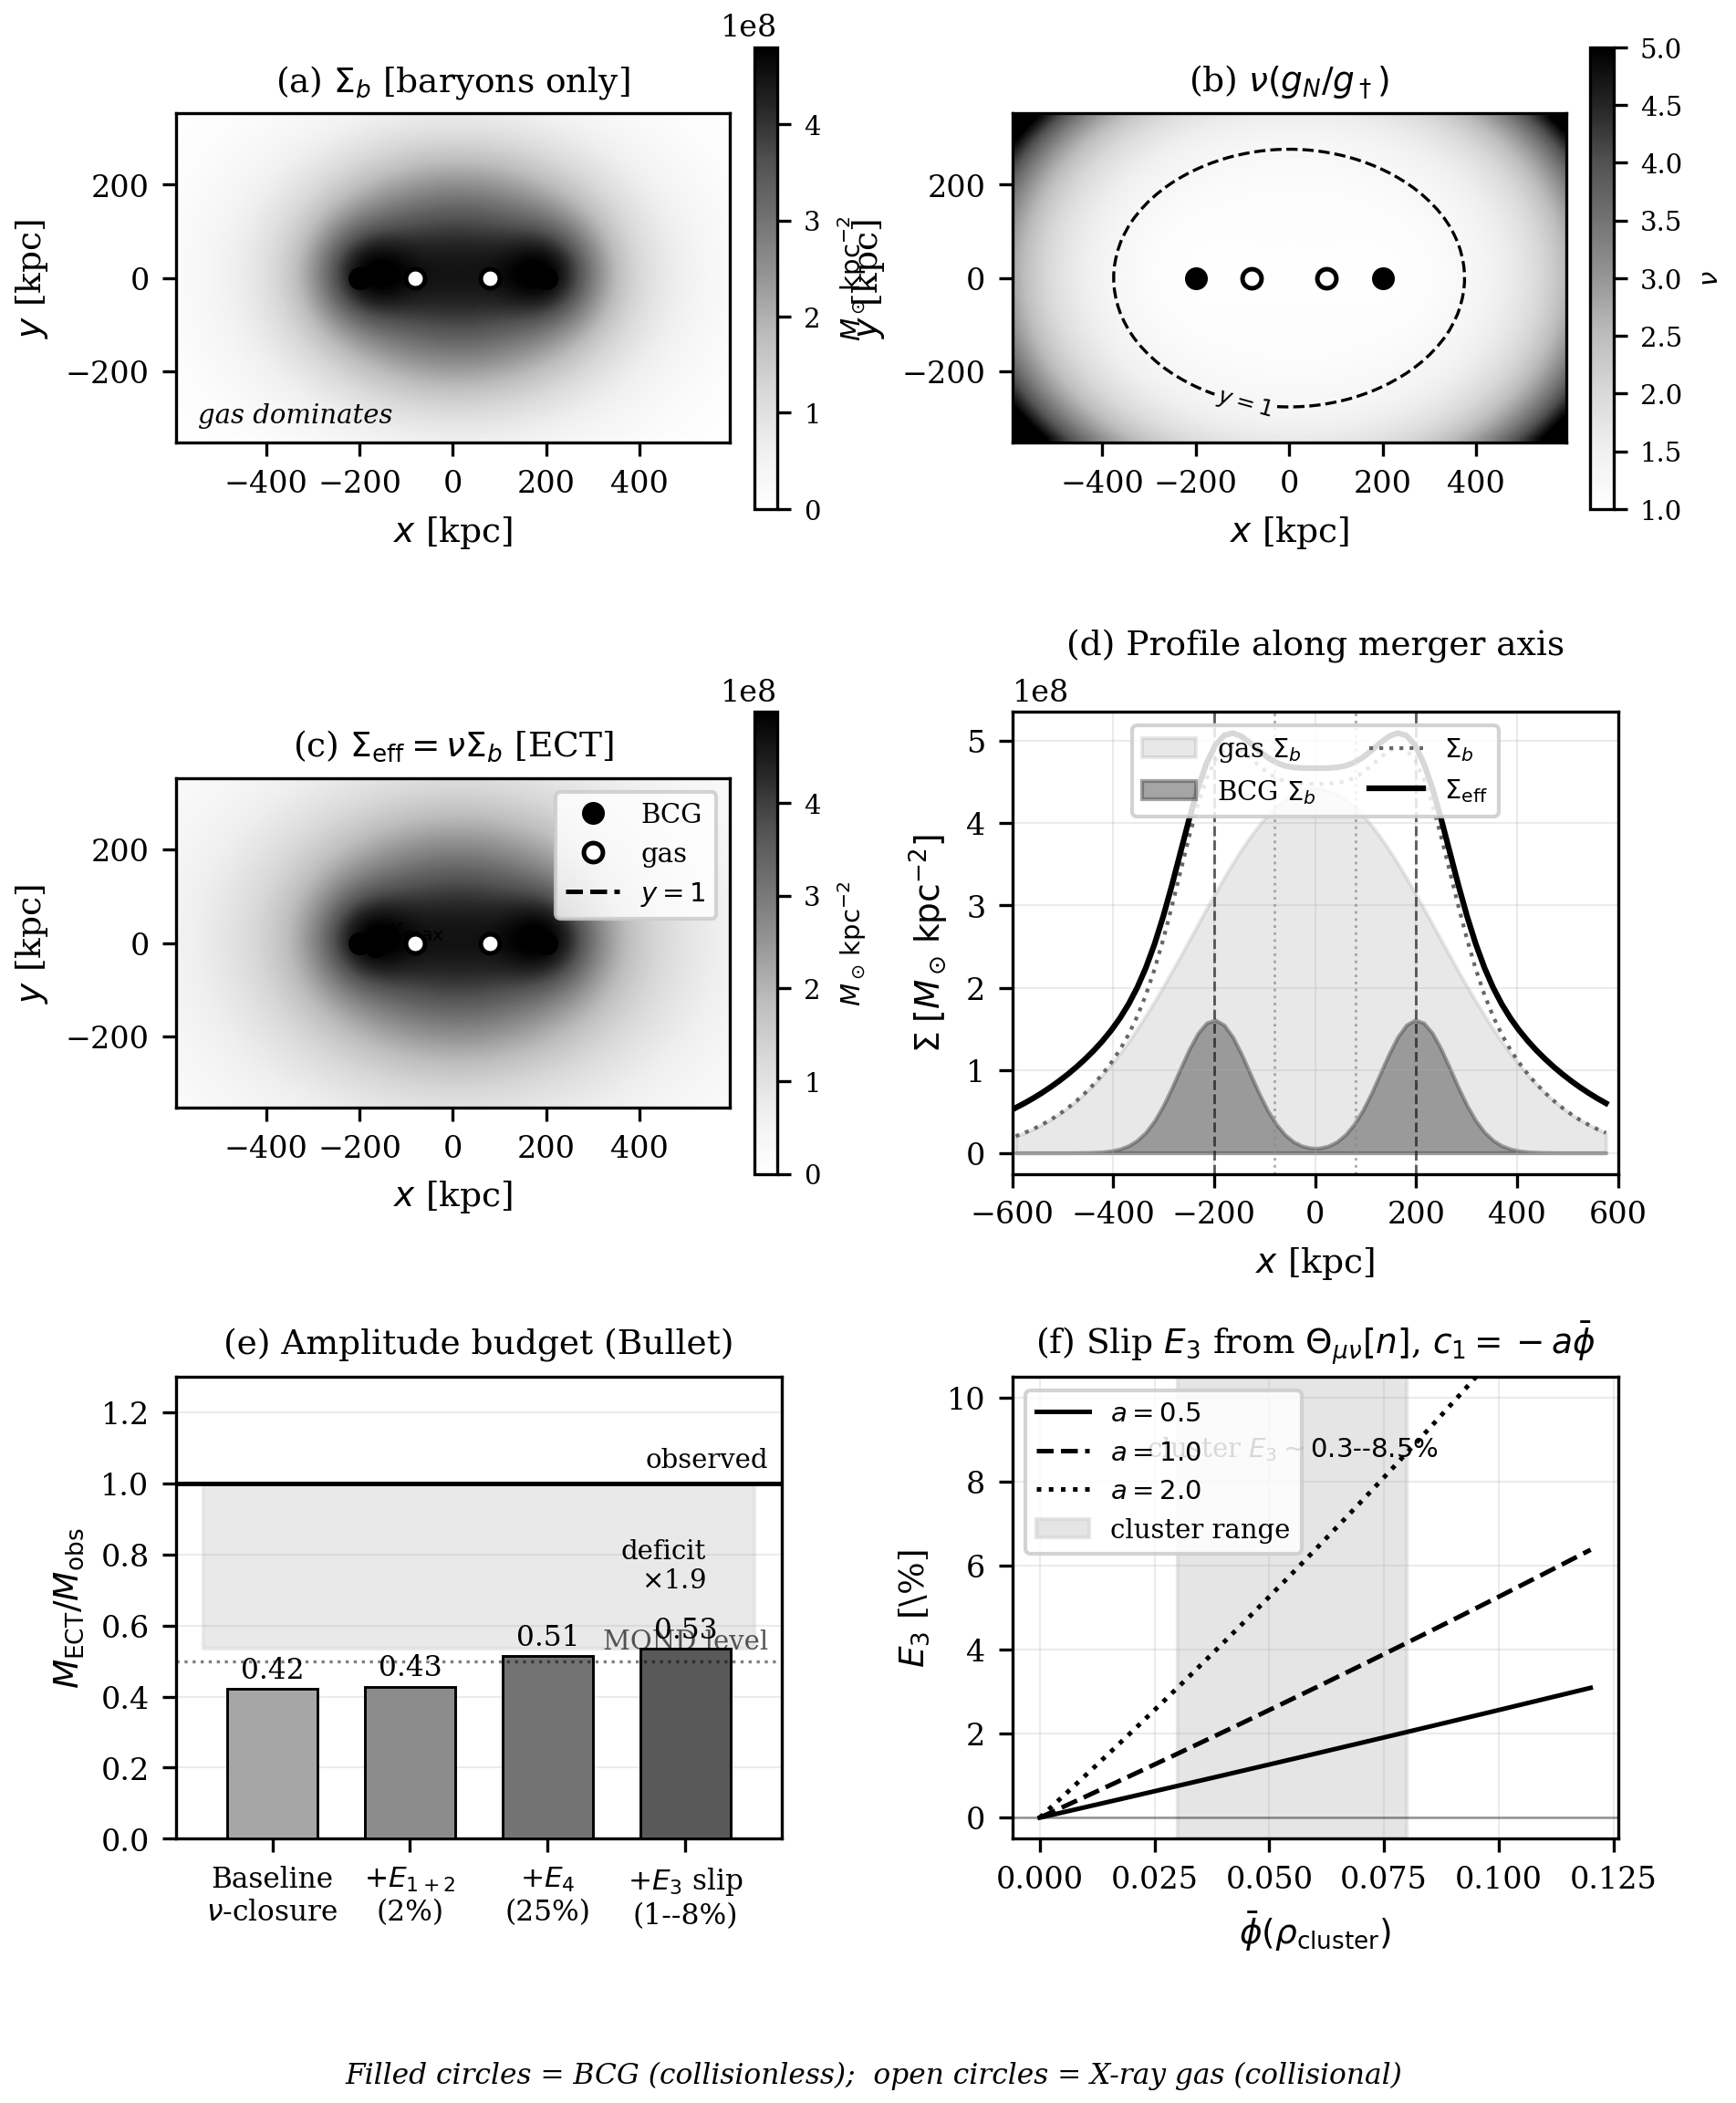
\includegraphics[width=0.82\textwidth]{fig_bullet_main.png}
\caption{Gravitational lensing in the Bullet Cluster (1E~0657-56). The lensing signal (contours) is offset from the X-ray gas (colour), conventionally attributed to collisionless dark matter. ECT reproduces this offset through the condensate $\phi$-closure without dark matter particles. (\emph{Level~B.})}
\label{fig:pop_bullet}
\end{figure}

\begin{figure}[H]
\centering
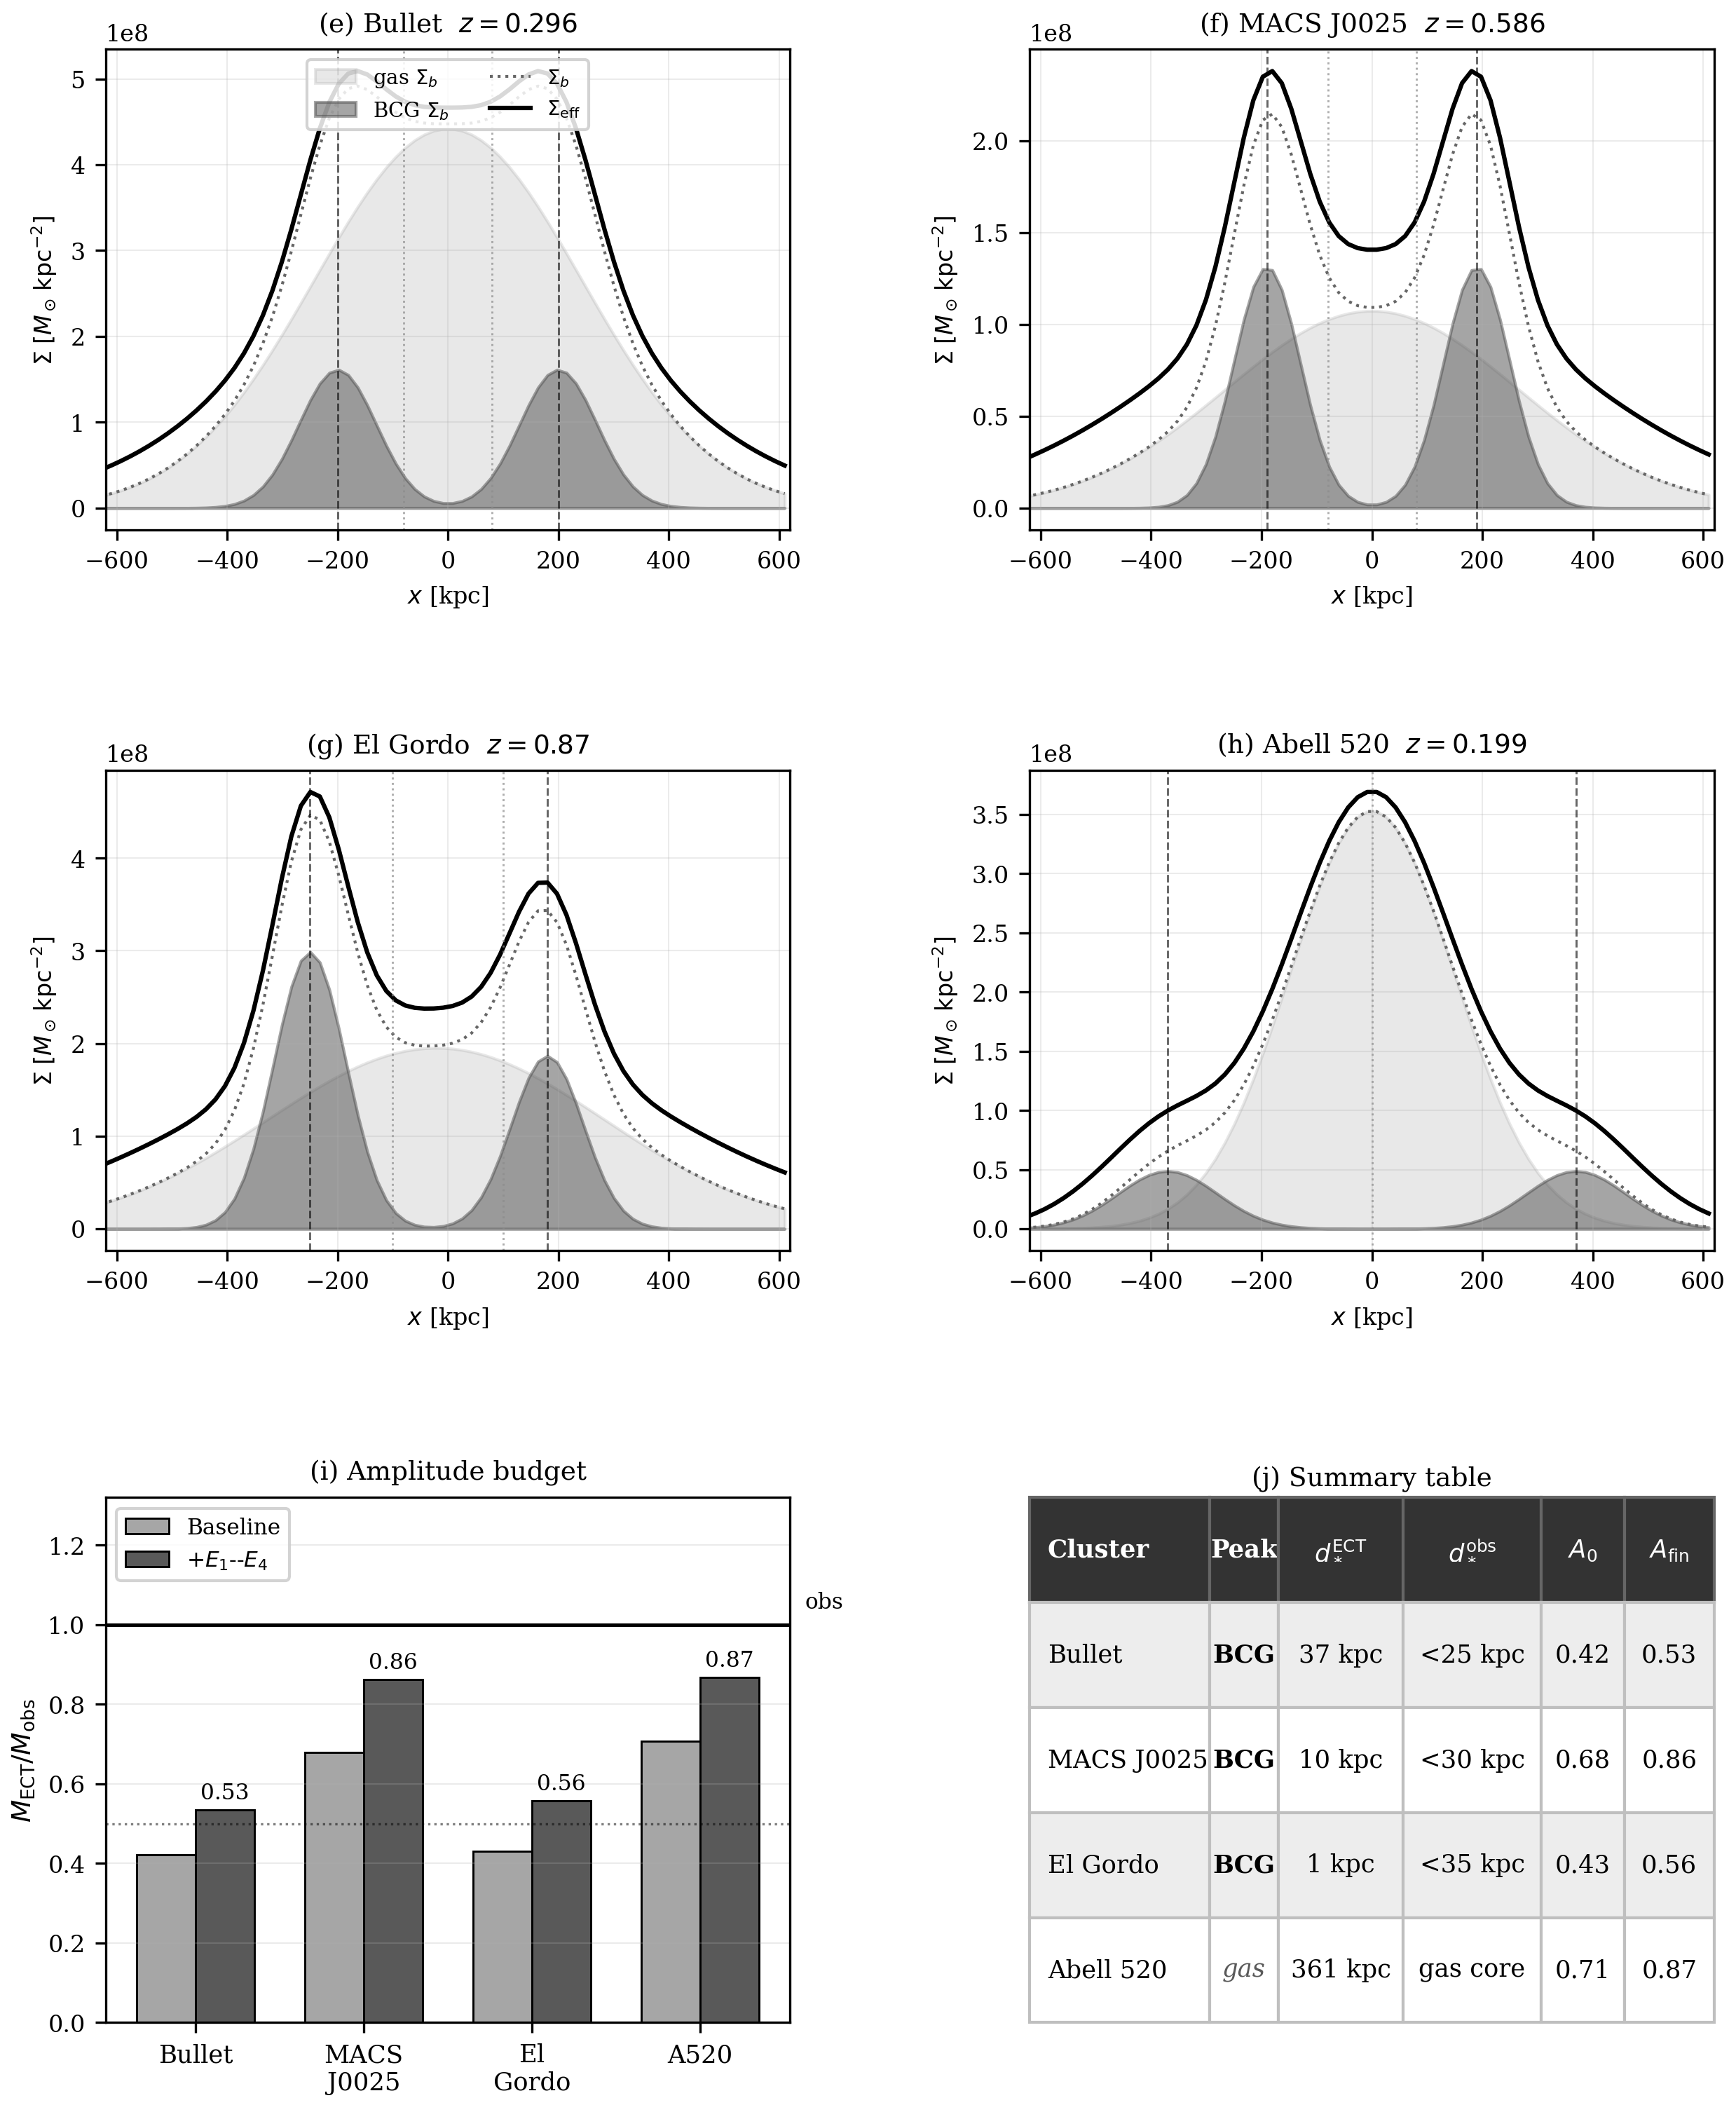
\includegraphics[width=\textwidth]{fig_cluster_suite_budget.png}
\caption{Cluster-merger gravitational lensing in ECT. Results for the Bullet Cluster, El Gordo, MACS~J0025, and Abell~520, including lensing mass ratios and morphology classification. In Abell~520, the lensing peak falls on the gas core --- consistent with ECT but a direct tension point for collisionless dark matter models. (\emph{Level~B.})}
\label{fig:pop_clusters}
\end{figure}

Galaxy-cluster mergers provide a critical dark-sector test. In a collision, the hot intracluster gas decelerates (electromagnetic interaction), while galaxies and any collisionless dark matter should pass through. In the Bullet Cluster, the lensing signal is offset from the gas toward the galaxies --- conventionally interpreted as evidence for collisionless dark matter halos.

ECT addresses cluster lensing through the $\phi$-closure with chameleon screening (Fig.~\ref{fig:pop_clusters}). The $\Theta_{\mu\nu}$ contribution generates gravitational slip, producing lensing morphology consistent with observations (\emph{Level~B}).

The case of \textbf{Abell~520} is particularly significant. In this system, the dominant lensing peak coincides with the \emph{gas-rich core}, not with the galaxy concentrations. This is a \emph{direct contradiction} to collisionless dark matter models, which predict that the lensing signal should track the collisionless component (galaxies). In ECT, this is the expected result: the gas core is locally more compact, so the $\phi$-enhancement is strongest there. A single rule generates galaxy-peaked lensing in Bullet/El~Gordo/MACS~J0025 and \emph{gas-peaked} lensing in Abell~520 --- a unified prediction absent in models requiring a fixed collisionless species.


\section{Matter--antimatter asymmetry}

The observable universe contains far more matter than antimatter: $\eta_B^{\rm obs} \approx 6 \times 10^{-10}$. This asymmetry requires baryon number violation, $C$/$CP$ violation, and departure from thermal equilibrium (the three Sakharov conditions, 1967). The Standard Model satisfies these conditions in principle but cannot quantitatively produce the observed asymmetry.

ECT provides a structural framework in which all three Sakharov conditions are satisfied by native ordered-medium mechanisms (\emph{Level~A} for the structural possibility). The $O(4) \to O(3)$ transition provides out-of-equilibrium conditions; the fifth coupling $\mathcal{L}_5$ supplies $CP$ violation; defect-mediated topology changes in the condensate allow baryon number violation. The specific leptogenesis mechanism and the estimated $\eta_B \sim 9 \times 10^{-10}$ (factor 1.5 from observation) are \emph{Level~B}.





\section{Conclusions of Part~II}

\subsection{Principal results}

From the ordered-branch EFT, the geometric branch produces:

\begin{enumerate}
\item Special Relativity as the homogeneous limit (\emph{A}).
\item GEE with $\Theta_{\mu\nu}[n]$ (\emph{B}).
\item Four cosmological problems resolved without inflation (\emph{A/B}).
\item Dynamical dark energy $w_0 \approx -0.83$ (\emph{B}).
\item Hubble tension: $\Delta H_0 \sim +3$\,km/s/Mpc (\emph{sign: A; magnitude: B}).
\item JWST early galaxies via enhanced $G_{\rm eff}$ + $\Theta_{\mu\nu}$ (\emph{B}).
\item 165 SPARC galaxies: $\chi^2/N \approx 2.95$ vs.\ $\Lambda$CDM 6.55 (\emph{B}).
\item BTFR slope exactly 4 (\emph{A}).
\item RAR: $g^\dagger \approx cH_0/(2\pi)$ (\emph{B}).
\item Cluster lensing incl.\ Abell~520 gas-peaked (\emph{B}).
\item Baryon asymmetry: Sakharov conditions natively (\emph{A/B}).
\item Dark matter and dark energy eliminated (\emph{B}).
\end{enumerate}

\subsection{Key equations and principles of Part~II}

Generalised Einstein equations: $G_{\mu\nu} + \Lambda_{\rm eff}g_{\mu\nu} = 8\pi G_{\rm eff}T_{\mu\nu} + \Theta_{\mu\nu}[n]$.

Galactic interpolation: $g(R) = \frac{1}{2}(g_N + \sqrt{g_N^2 + 4g_Ng^\dagger})$.

BTFR: $v_{\rm flat}^4 = G_N M_{\rm bar} g^\dagger$ (slope 4, algebraic).

$G_{\rm eff}(z) \approx G_N(1+z)^{2\varepsilon}$, $\varepsilon \approx 0.01$ (Hubble shift).

\subsection{Observational tests and falsifiers}

ECT is falsifiable. Key predictions of the macroscopic sector:

\begin{itemize}
\item BTFR slope = 4 (\emph{A}); $g^\dagger \propto cH_0$ (\emph{B}).
\item Fifth force $\eta \sim 10^{-15}$ (\emph{B}); dark energy $w_0 \approx -0.83$ (\emph{B}).
\item Environmental $g^\dagger$ modulation (\emph{B}); $M_{\rm max} = 2.17\,M_\odot$ (\emph{B}).
\item CMB quadrupole deficit (\emph{B/Open}).
\end{itemize}
Full list with explanations is given in Part~IV, Section~\ref{sec:pop_predictions}.

\begin{figure}[H]
\centering
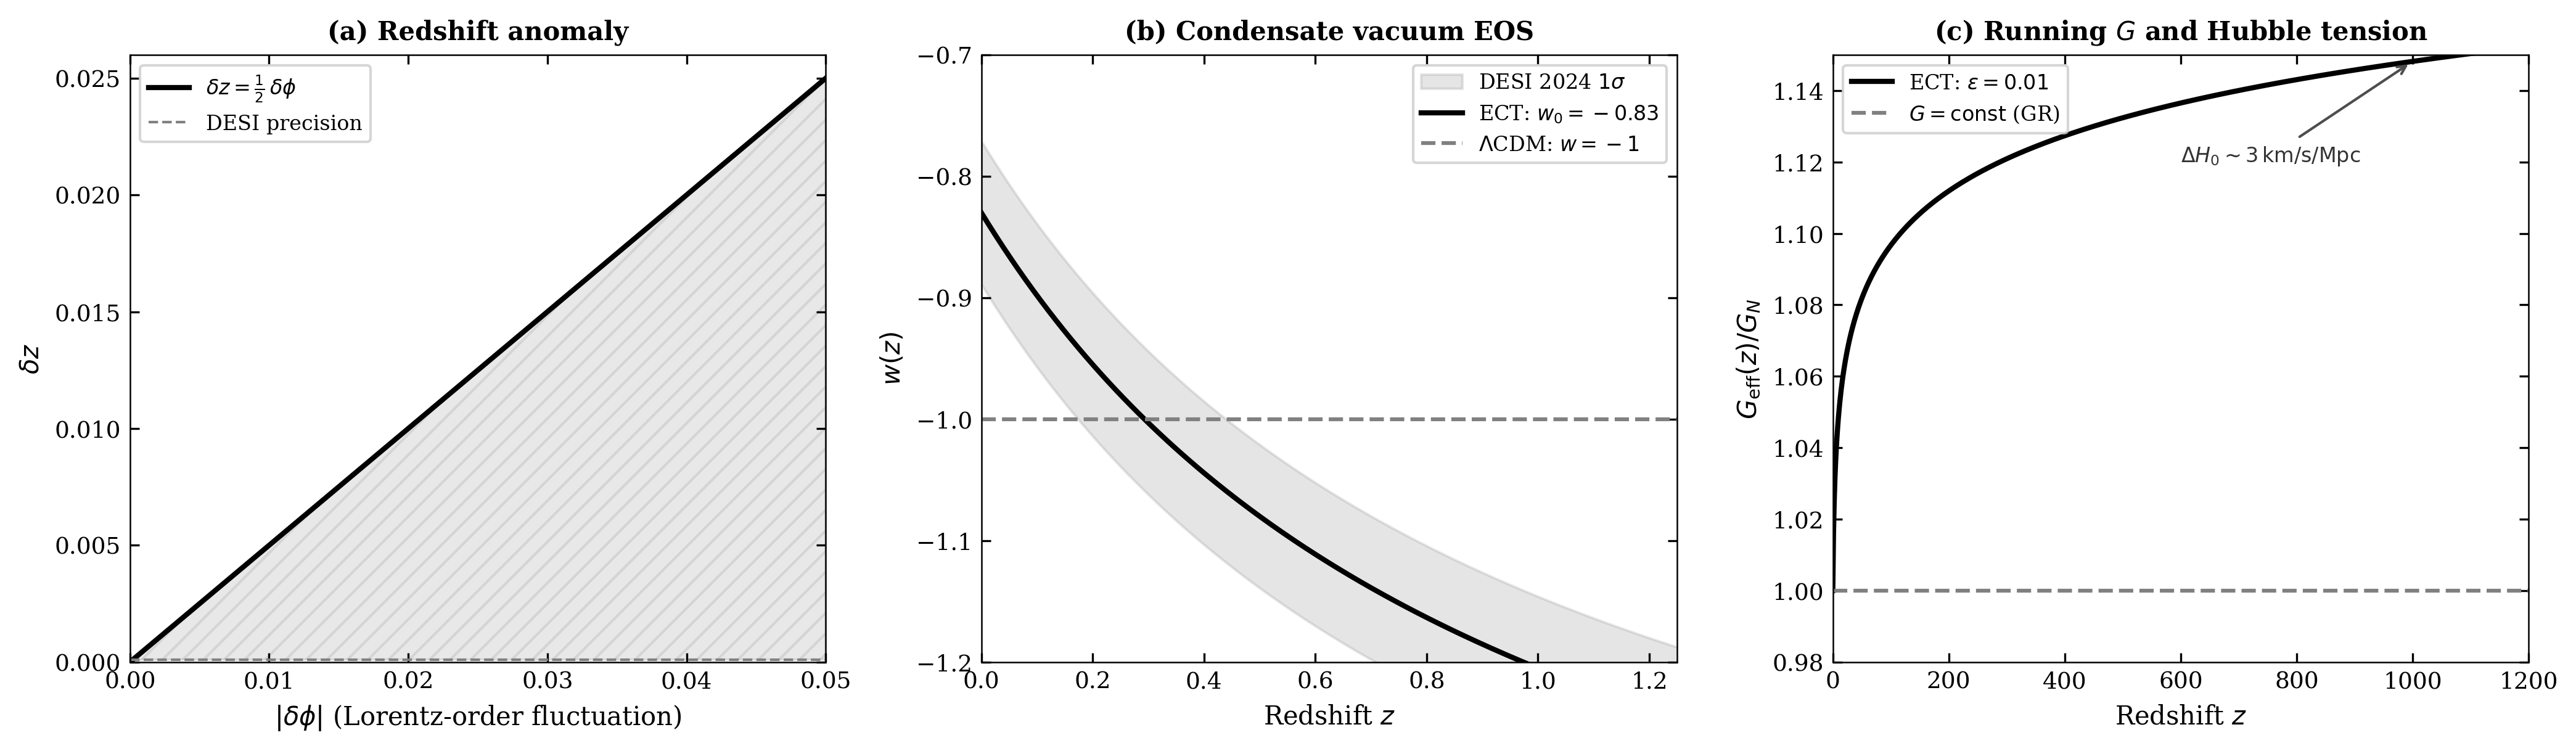
\includegraphics[width=0.88\textwidth]{fig_cosmo_predictions.png}
\caption{ECT cosmological predictions and comparison with observations and $\Lambda$CDM. ECT provides correlated predictions for dark energy, the Hubble tension, the JWST problem, and galactic phenomenology from the same ordered-branch dynamics. (\emph{Level~B.})}
\label{fig:pop_preds}
\end{figure}

\subsection{Part~II derivation logic}

\begin{figure}[H]
\centering

\includegraphics[width=\textwidth]{fig_partII_derivation_logic_pop.pdf}
\caption{Part~II derivation logic. From the ordered-branch EFT, the geometric branch produces all macroscopic results listed above. Colours indicate derivation levels.}
\label{fig:pop_partII_logic}
\end{figure}

The full derivation logic of Part~II is shown in Fig.~\ref{fig:pop_partII_logic}. The cosmological predictions are summarised in Fig.~\ref{fig:pop_preds}.

%==============================================================
\part{Quantum Sector: Coherent Branch}
\label{part:quantum_pop}

\noindent\textbf{Why does quantum mechanics exist?} In ECT, the answer has three layers.

\emph{First}: the Euclidean functional integral. Because the fundamental arena is a four-dimensional Euclidean manifold with no built-in time, the natural mathematical object is the functional integral $\int \mathcal{D}\Phi\,e^{-S_E[\Phi]}$, which sums over \emph{all} field configurations --- including ``closed histories'' where the field returns to itself along the fourth coordinate. There are no events, no temporal ordering, no cause-effect sequences at this level. By the Osterwalder--Schrader reconstruction theorem, this Euclidean functional integral is mathematically equivalent to a unitary quantum theory on a Hilbert space (\emph{Level~A/B}).

\emph{Second}: the action scale $S_0 = \hbar$. The compact phase $\theta$ of the condensate ($\Phi_{\rm eff} = \rho\,e^{i\theta}$) imposes single-valuedness on closed loops: $\oint \partial_A\theta\,dX^A = 2\pi n$. This topological constraint sets the minimal loop action $S_{\rm loop,min} = 2\pi S_0$, where $S_0$ is identified with $\hbar$ through the condensate matching relation (\emph{Level~B}).

\emph{Third}: the physical interpretation of the Euclidean--Lorentzian boundary. In the Euclidean regime, all configurations contribute coherently to the functional integral --- including closed histories that would be ``forbidden'' in the Lorentzian sense. After the emergence of the Lorentzian causal structure, these closed histories continue to contribute to quantum amplitudes: they are the source of interference, superposition, and tunnelling. For macroscopic systems with $N_{\rm eff} \gg 1$, decoherence exponentially suppresses the coherent contribution of these closed Euclidean histories, and classical behaviour emerges. For microscopic systems with $N_{\rm eff} \sim 1$, the closed histories remain coherent --- this is quantum behaviour. The quantum--classical boundary is therefore not a separate postulate but a consequence of the number of environmental modes coupled to the system (\emph{Level~A/B}).


\section{ECT versus standard quantum mechanics}
\label{sec:pop_ect_vs_qm}

\begin{figure}[H]
\centering
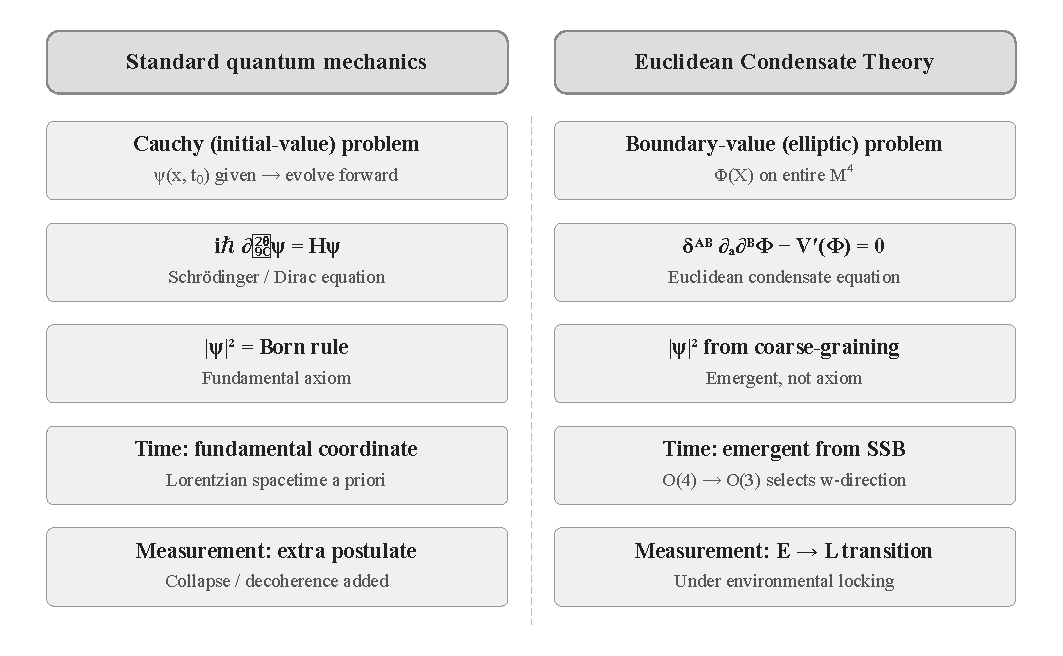
\includegraphics[width=0.75\textwidth]{fig_ect_vs_qm.pdf}
\caption{Structural comparison of standard quantum mechanics (left) and ECT's coherent branch (right). Standard QM starts from axioms (Hilbert space, operators, Born rule, Schr\"odinger equation) and computes predictions. ECT derives these structures from the Euclidean condensate dynamics. The central column shows the structural origins that ECT provides for each axiom. (\emph{Level~A/B for the structural routes; Level~Open for the fully closed Born theorem.})}
\label{fig:pop_ectvqm}
\end{figure}

Standard quantum mechanics answers the question ``how?'': given a Hamiltonian and an initial state, it prescribes how to compute probabilities. ECT aims to answer the additional question ``why?'': why do Hilbert spaces, operators, superposition, the Born rule, and decoherence exist at all? (Fig.~\ref{fig:pop_ectvqm}).

The deepest structural distinction lies in the type of mathematical problem. In standard QM, the fundamental problem is the \emph{Cauchy problem} (initial-value problem): $i\hbar\,\partial_t\psi = H\psi$. Given the state at $t=0$, time evolution uniquely propagates it forward. In ECT, the fundamental problem is a \emph{boundary-value problem} on the Euclidean manifold: $\delta^{AB}\partial_A\partial_B\Phi - V'(\Phi) = 0$. The solution is constrained by data on the \emph{entire boundary} of the four-dimensional domain, not just on one time-slice.

This has profound consequences. The Cauchy problem generates \emph{one-directional} evolution: past determines future, but not vice versa. The boundary-value problem generates a \emph{four-dimensionally self-consistent} configuration: future boundary conditions constrain the present just as past boundary conditions do. This is not retrocausality in the Lorentzian sense --- it is the normal functioning of a boundary-value problem. The probabilistic character of quantum mechanics, in ECT's view, arises not from fundamental indeterminacy but from coarse-graining: when untracked environmental modes are integrated out, the effective description of a subsystem becomes inherently statistical.


\subsection{Detailed structural comparison: ECT vs standard QM}

The following comparison illustrates how ECT's coherent branch differs from standard quantum mechanics on specific physical examples.

\textbf{The hydrogen atom.} In standard QM, one solves $H\psi = E\psi$ and obtains $E_n = -13.6/n^2$\,eV together with the probability densities $|\psi_{nlm}|^2$. In ECT, the hydrogenic spectrum arises from the four-dimensional Euclidean field equation for $\Phi$ together with the self-consistency condition in the $w$-direction expressed by single-valuedness: $\oint dw \cdot p_w = 2\pi S_0\,n$. The discrete spectrum is associated with self-consistency conditions on admissible condensate configurations, rather than with eigenvalues of a fundamentally probabilistic wave equation (\emph{Level~B}).

\textbf{The double-slit experiment.} In standard QM, $\psi = \psi_1 + \psi_2$ and $P = |\psi_1 + \psi_2|^2$. In ECT, the interference pattern arises from one connected solution of the underlying elliptic boundary-value problem, whose effective Lorentzian projection contains contributions associated with both slit channels. The interference is a property of the four-dimensional field configuration, not of an abstract probability wave (\emph{Level~A/B}).

\textbf{Measurement.} In standard QM, collapse is an extra postulate. In ECT, the detector belongs to the full boundary-value problem. At the reduced-description level, effective collapse is the subsystem manifestation of a Euclidean-to-Lorentzian transition under strong environmental locking ($\Gamma_{\rm loop} \gtrsim 1$). Multiple winding sectors coexist in the coherent regime; environmental coupling drives decoherence; when $\Gamma_{\rm loop} \gg 1$, interference is suppressed and a single classical outcome is selected (\emph{Level~A/B}).

\textbf{Determinism.} The fundamental Euclidean equation is deterministic: one specifies boundary conditions and obtains one global field configuration. No probabilities, no collapse, no stochasticity at the deepest level. Statistical quantum mechanics appears because realistic observers never have access to the full condensate state. When environmental modes are integrated out, the subsystem acquires influence functionals, reduced density matrices, and effective probabilities. ECT stands to standard QM as microscopic Newtonian mechanics stands to statistical mechanics: deterministic underneath, probabilistic after coarse-graining (\emph{Level~A}).

\textbf{``Future affects past.''} In standard QM, this does not arise because the theory is formulated as a forward-time Cauchy problem. In ECT, it is natural: for an elliptic equation, changing the boundary condition on one side changes the solution throughout the domain, including what the Lorentzian reading would call the ``past'' side. This is the structural reason why delayed-choice phenomena are naturally accommodated (\emph{Level~A/B}).

\textbf{Unified origin of coherent and geometric branches.} A central structural claim of ECT: gravity and quantum coherence are not separate ingredients forced together, but two sectors of one ordered condensate. The long-wavelength sector is read geometrically (gravity); the coherent shorter-wavelength sector is read wave-mechanically (quantum). This is not ad hoc stitching --- it follows from the mode decomposition of the same condensate around the same ordered background (\emph{Level~A}).

\textbf{What ECT already reproduces:} (i)~Schr\"odinger equation as non-relativistic limit; (ii)~Klein--Gordon from ordered branch; (iii)~action quantisation through $S_0$ and phase compactness; (iv)~decoherence and quantum--classical boundary; (v)~Euclidean-to-Lorentzian measurement reading; (vi)~spin discretisation from $O(3)$; (vii)~PES for persistent-state selection; (viii)~gravitational decoherence; (ix)~unified tunnelling and entanglement; (x)~cross-sector $S_0$ universality.

\textbf{What remains open:} Born rule from first principles; complete measurement theorem; Bell correlators from condensate theory; three generations; $\alpha_{\rm fs} = 1/137$; full Yukawa hierarchy. These are open derivational targets, not failures of the framework.


\section{Hilbert-space structure from reflection positivity}

One of the central results of Part~III is the reconstruction of Hilbert-space structure from Euclidean data, using the mathematical tool of \textbf{reflection positivity} (RP). If the Euclidean two-point function satisfies RP (a property proved for the ordered-branch correlator), the Osterwalder--Schrader reconstruction theorem (1975) guarantees the existence of a Hilbert space $\mathcal{H}$ with a positive-definite inner product, a self-adjoint Hamiltonian generating unitary time evolution, and canonical commutation relations $[q,p]=i\hbar$ (\emph{Level~A/B}).

Standard QM uses the Osterwalder--Schrader theorem in the \emph{opposite} direction: starting from a quantum theory, it checks that the Euclidean continuation is well-defined. ECT uses it \emph{constructively}: starting from the Euclidean condensate, it \emph{builds} the Hilbert space. The quantum formalism is constructed, not assumed.


\section{Superposition, interference, exchange statistics, and the Pauli exclusion principle}

\textbf{Superposition} (\emph{Level~A/B}): The linearised fluctuation equation in the coherent branch is linear. Solutions can be added, producing superposition without any axiom.

\textbf{Interference} (\emph{Level~A}): Arises from the compact-phase structure. Paths with different phase accumulations contribute to the functional integral with different factors $e^{iS/\hbar}$, producing constructive or destructive combination --- the same mechanism that produces interference in a superfluid.

\textbf{Indistinguishability of same-species particles}: In ECT, particles of the same species are quanta of the same emergent mode sector of the same ordered medium. There is no hidden individuation label; exchange reassigns occupation rather than permuting individuated objects. The many-particle configuration space is therefore already the quotient by exchange.

\textbf{Exchange statistics} (\emph{Level~A/B}): Connected to the topology of path configurations in the Euclidean manifold. Paths that exchange identical particles acquire a factor $+1$ (bosons) or $-1$ (fermions) depending on the topological class of the exchange. The spin-statistics connection (integer spin $\leftrightarrow$ bosons, half-integer $\leftrightarrow$ fermions) is structurally motivated (\emph{Level~A/B}); a fully rigorous derivation from bare P3 remains open.

\textbf{Pauli exclusion principle} (\emph{Level~A/B}): For fermions, the $-1$ exchange factor means that configurations with two identical fermions in the same state contribute with opposite signs and cancel. Pauli exclusion is a consequence of exchange topology, not a separate axiom.

In standard QM, all four of these properties are either postulated directly or follow from operator axioms that are themselves postulated. In ECT, they arise from the geometry and topology of the ordered condensate.


\section{The Principle of Euclidean Stationarity}
\label{sec:pop_pes}

\begin{figure}[H]
\centering
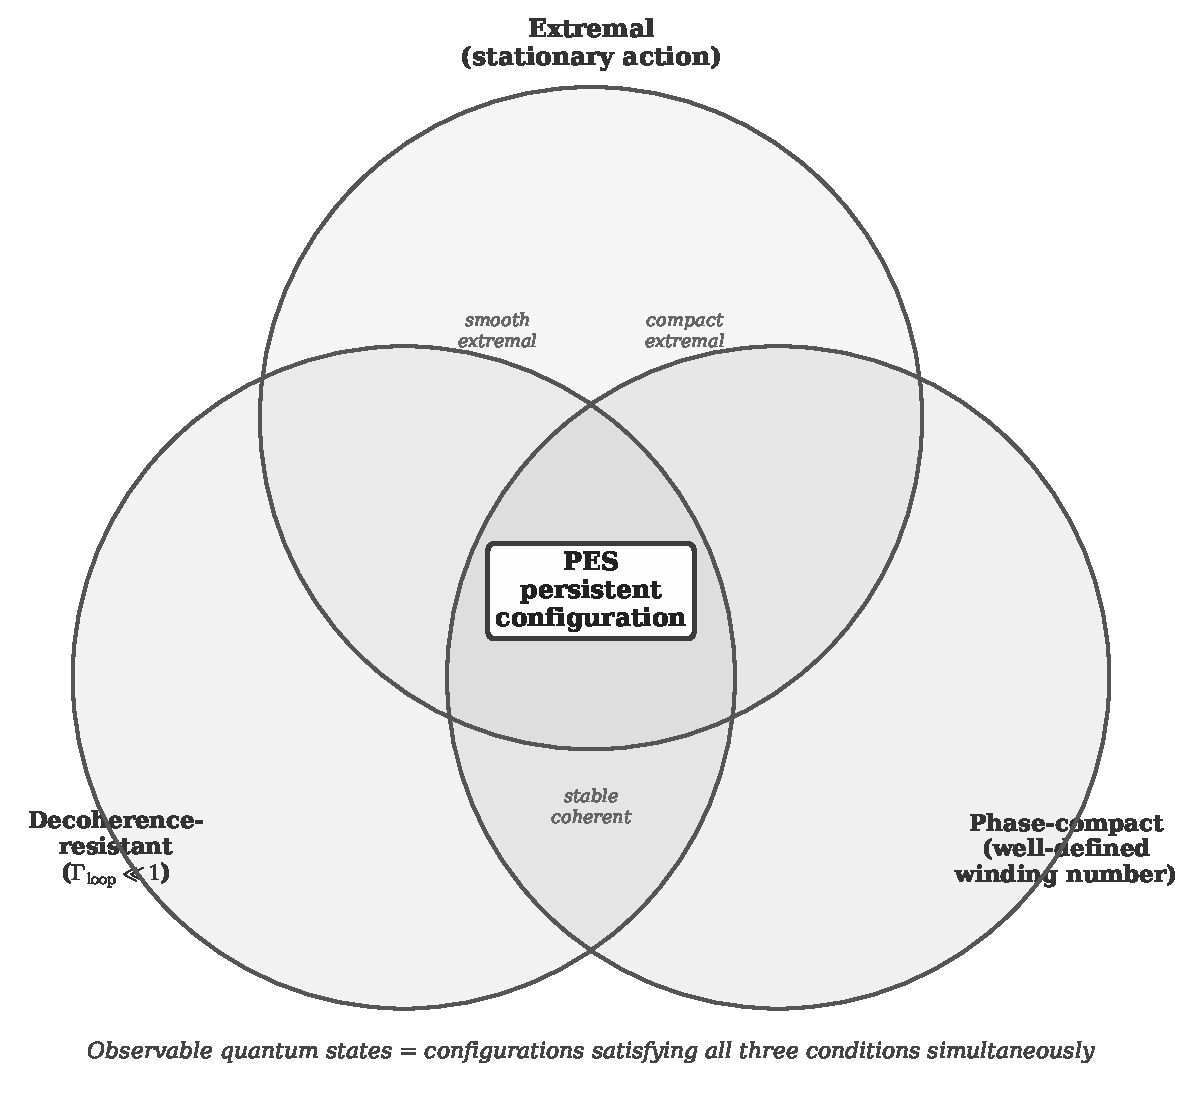
\includegraphics[width=0.65\textwidth]{fig_pes_diagram.pdf}
\caption{The Principle of Euclidean Stationarity (PES). Three conditions must be simultaneously satisfied: the configuration is an extremal of the Euclidean action (stationary), it is resistant to environmental decoherence ($\Gamma_{\rm loop}\ll1$), and it belongs to a well-defined phase-topological class (compact phase with integer winding). Their intersection defines the persistent configurations --- the ECT counterpart of observable quantum states. (\emph{Level~B.})}
\label{fig:pop_pes}
\end{figure}

The Principle of Euclidean Stationarity (PES) is a key organising principle of ECT (Fig.~\ref{fig:pop_pes}). It is not a new postulate but an organising principle that emerges as a consequence of three already-established ingredients: the Euclidean-first ontology (P1), the compact-phase topology (BR1), and the influence-functional decoherence framework.

\textbf{Statement.} The physically persistent and observable configurations are those that simultaneously: (i)~are stationary or quasi-stationary extremals of the Euclidean action; (ii)~maintain $\Gamma_{\rm loop} \ll 1$ (resist decoherence); (iii)~belong to an admissible phase-topological class (integer winding). Configurations failing any of these conditions decohere and are absorbed into the classical branch.

\textbf{Physical consequences.} PES explains \emph{why} quantum systems settle into energy eigenstates: these are precisely the Euclidean-stationary configurations that survive environmental coupling. After the Wick rotation $w \to -ic_*t$, a Euclidean-stationary configuration with action $S_E$ corresponds to an energy eigenstate with energy $E = S_E/\Delta w$. The ground state corresponds to the lowest-action Euclidean extremal.

\textbf{Relation to the principle of least action.} PES is more fundamental than the classical principle of least action. The latter is the $\Gamma_{\rm loop} \gg 1$ limit of PES: when decoherence is strong, only the single lowest-action path survives, and classical mechanics emerges. PES thus \emph{contains} the principle of least action as a limiting case while also explaining quantum behaviour.

\textbf{Relation to discreteness.} The discreteness of atomic spectra, quantised energy levels, and all integer quantum numbers follow from PES: only integer-winding, action-stationary, decoherence-resistant configurations survive. This replaces the Bohr postulate (integer quantum numbers) with a structural selection mechanism.


\section{Probability, the Born rule, and measurement}

In standard quantum mechanics, the Born rule $P = |\psi|^2$ is a foundational axiom. In ECT it is not postulated but motivated as a consequence of decoherence: when the influence functional suppresses interference between branches, the remaining branches behave as classical alternatives whose weights are determined by the squared amplitude. The Born rule is structurally supported through the reflection-positive inner product (\emph{Level~B}): in the Hilbert space constructed via Osterwalder--Schrader, the squared modulus of the transition amplitude is automatically positive and normalised.

More broadly, ECT does not merely reinterpret the axioms of quantum mechanics; it changes their logical status from foundational postulates to reconstruction targets: Hilbert space is constructed (not postulated), unitarity follows from reflection positivity, the Born rule is motivated by decoherence, and ``collapse'' is identified with the Euclidean-to-Lorentzian transition at $\Gamma_{\rm loop}\sim 1$---no mystical observer is invoked.

The measurement problem --- why does a quantum superposition appear to ``collapse'' upon measurement? --- is addressed through decoherence (\emph{Level~A/B}). The interaction between the measured system, the apparatus, and the condensate environment rapidly suppresses off-diagonal terms in the density matrix, producing effective collapse. No additional collapse postulate is needed. What remains open is a fully closed mathematical theorem deriving the Born rule without any extra closure input (\emph{Level~Open}).


\section{Quantum entanglement and Bell correlations}
\label{sec:pop_entanglement}

In standard QM, entanglement is a primitive property of the tensor-product Hilbert space. In ECT, it is a structural feature of the Euclidean condensate (\emph{Level~A/B}).

In the coherent branch, subsystems are not fundamental isolates --- they are reduced sectors of a single ordered medium. Two subsystems sharing a common condensate with $\Gamma_{\rm loop} \ll 1$ are correlated through the Euclidean substrate without requiring Lorentzian signalling. Four-dimensional Euclidean coherence produces non-local (in the 3D Lorentzian sense) correlations: correlations that would be surprising if one thinks in terms of 3D local causality, but are entirely natural as correlations within a single 4D Euclidean field configuration.

ECT does not violate Bell's theorem: it is not a local hidden-variable theory. The ``non-locality'' of entanglement is reinterpreted as common-medium correlation in the Euclidean arena, consistent with the no-signalling theorem. Two subsystems are entangled not because a hidden superluminal signal connects them, but because both are partial descriptions of one and the same coherent condensate configuration. Measurement of one part does not ``send an influence'' to the other; it converts the local subsystem into a decohered branch, while the other was already part of the same global configuration. The observed correlation reflects prior inseparability, not signal transfer. A full first-principles derivation of Bell-inequality-violating correlators and Tsirelson bounds remains open (\emph{Level~Open}).

\textbf{Delayed-choice experiments} (Wheeler) receive a natural interpretation. In the boundary-value problem of ECT, future detector settings are part of the boundary data that constrain the Euclidean field configuration globally. This is not retrocausality --- it is the standard behaviour of a boundary-value problem.


\section{Tunnelling}

In standard QM, quantum tunnelling --- the ability of a particle to traverse a classically forbidden barrier --- is a consequence of wave mechanics, but its physical mechanism is mysterious. In ECT, tunnelling has a clear geometric interpretation (\emph{Level~A/B}).

In the Euclidean picture, a ``classically forbidden'' region corresponds to a region where the Lorentzian kinetic energy would be negative. But in the Euclidean domain, all four directions are equivalent --- there is no distinction between ``classically allowed'' and ``classically forbidden.'' The field configuration simply passes through the barrier in the four-dimensional Euclidean space. After the Wick rotation, this Euclidean passage manifests as exponentially suppressed but nonzero amplitude on the other side of the barrier --- tunnelling.

This is the same logic used in the standard instanton calculation, but ECT gives it an ontological reading: tunnelling is not a ``mysterious quantum effect'' but a natural consequence of the fact that the fundamental arena is Euclidean, and classically forbidden regions are an artefact of the Lorentzian projection. At the present level, the standard WKB/instanton suppression is quantitatively recovered; the gain is primarily interpretive and geometric, not yet an established distinct numerical deviation.


\section{Interactions belong to the Lorentzian branch}

A conceptually important distinction in ECT is that \emph{interaction} --- in the sense of one physical system exchanging energy, momentum, or information with another --- is fundamentally a Lorentzian concept (\emph{Level~A}).

In the coherent branch ($\Gamma_{\rm loop} \ll 1$), what exists is not interaction but \emph{common-medium correlation}: subsystems share a coherent condensate configuration, and their effective descriptions are correlated through the Euclidean substrate. No energy exchange occurs; no signal is transmitted; no ``event'' in the Lorentzian sense takes place.

Interaction requires decoherence: one subsystem must couple to another strongly enough that $\Gamma_{\rm loop}$ crosses the threshold $\sim 1$. At that point, the coherent correlations are converted into classical, Lorentzian, causal events --- energy is exchanged, momentum is transferred, information is communicated. Measurement, in this picture, is the process that converts Euclidean common-medium correlation into Lorentzian interaction.

This does not mean there is no coupling at all. The influence of the medium enters through the influence functional; the decoherence kernel, medium response, and suppression of off-diagonal elements are all consequences of the medium, not of ``forces'' in the Lorentzian sense. The correct distinction is not ``interaction versus no interaction'' but ``decohered Lorentzian event-like interaction versus Euclidean common-medium correlation.''

This separation explains why quantum systems can exhibit non-local correlations (entanglement) without violating causality: the correlations belong to the coherent Euclidean branch, while causal signalling belongs to the decoherent Lorentzian branch.


\section{Influence of future boundary conditions}
\label{sec:pop_future}

Because the fundamental ECT equation is a boundary-value problem on the Euclidean manifold (not a Cauchy problem), boundary data on \emph{all} sides of the domain constrain the solution. After the Wick rotation to Lorentzian signature, this means that future boundary conditions can constrain the present configuration.

This is not backward-in-time causation in the Lorentzian sense. It is the standard mathematical property of boundary-value problems: the solution at any interior point depends on data everywhere on the boundary. Global Euclidean boundary-value dependence is not retro-signalling within Lorentzian spacetime; no Lorentzian causality violation is implied. In ECT, this property provides a natural framework for understanding delayed-choice experiments, quantum eraser phenomena, and the apparent ``retrocausal'' features of the two-state vector formalism (\emph{Level~A/B}).


\section{Quantum vacuum effects}

The ordered condensate is not an empty backdrop but a physically active medium. Its response to boundaries, acceleration, and cosmological expansion produces three classes of observable effects:

\textbf{The Casimir effect} (\emph{Level~B, conditional}): In standard QED, the Casimir force between conducting plates arises from modified vacuum fluctuation modes. In ECT, the ordered vacuum can in principle respond to boundaries that reflect its soft orientation sector, not just the photon sector. Within a provisional multi-component soft-orientation EFT with idealised condensate-reflecting Dirichlet boundaries, a naive counting argument yields an enhancement factor of $3/2$ relative to QED. However, this provisional factor depends on boundary conditions that standard metallic plates do not implement (the neutral soft sector couples to matter only gravitationally), and on a three-component coordinate counting that the integrability constraint of the scalar-only basis reduces at the physical level ($N_G^{\rm phys}=1$ at linear order). The $3/2$ ratio is therefore conditional, boundary-sensitive, and model-dependent---not a universal laboratory prediction. What is structurally robust (Level~A) is the claim that a nontrivial ordered vacuum must be boundary-sensitive.

\textbf{The Unruh effect} (\emph{Level~A/B}): An accelerated observer in the ECT vacuum perceives a thermal bath with temperature $T = \hbar a/(2\pi c k_B)$, identical to the standard prediction. The derivation traces this to the analytic continuation from the Euclidean frame to the Rindler frame.

\textbf{Cosmological particle production} (\emph{Level~B}): At the $O(4) \to O(3)$ phase transition, the abrupt change in the condensate background creates real particle--antiparticle pairs. In ECT this is not the mysterious ``appearance of something from nothing'': modes that were ``quiet'' in the symmetric phase cease to be quiet in the ordered phase because the background against which ``silence'' is defined has changed---analogous to the production of phonons when a superfluid is rapidly cooled.


\section{Decoherence and the quantum--classical boundary}

\begin{figure}[H]
\centering
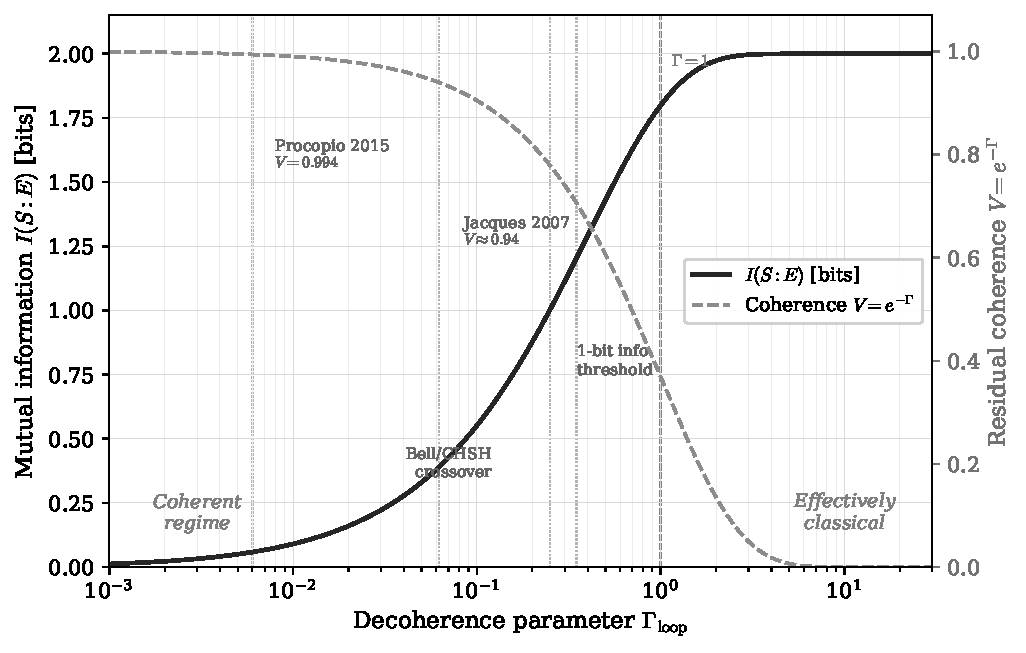
\includegraphics[width=0.78\textwidth]{fig_qubit_info_decoherence.pdf}
\caption{Decoherence regimes in ECT. The information content of a quantum system evolves differently depending on the environmental coupling strength $N_{\rm eff}\gamma$. For weak coupling (quantum regime), coherence is preserved. For strong coupling (classical regime), off-diagonal density matrix elements are exponentially suppressed. (\emph{Level~A/B.})}
\label{fig:pop_qubit}
\end{figure}

ECT provides a unified influence-functional framework for decoherence (Fig.~\ref{fig:pop_qubit}), treating both environmental and gravitational channels through the same mathematical structure (\emph{Level~A/B}).

\textbf{Environmental decoherence}: interaction with thermal photons, air molecules, phonons, and other environmental degrees of freedom.

\textbf{Gravitational decoherence}: interaction with the condensate orientation field $n^A$. This is an ECT-specific prediction: the condensate itself acts as a universal decoherence bath, even in the absence of ordinary matter environments.

The decoherence time is $\tau_{\rm dec} = 1/(N_{\rm eff}\gamma)$, where $N_{\rm eff}$ is the number of effective environmental modes and $\gamma$ is the coupling rate. Numerical estimates: free electron in vacuum, $\tau_{\rm dec} \gg 10^{10}$\,yr; fullerene C$_{60}$, $\tau_{\rm dec} \sim 10^{-6}$\,s (consistent with observed interference); dust grain in air, $\tau_{\rm dec} \sim 10^{-15}$\,s.

\textbf{Physical picture.} In ECT, decoherence is not a postulate about observers destroying wave functions. It is a physical process: the subsystem loses its coherent integrity because it couples to a large number of condensate degrees of freedom that it cannot track. No separate collapse postulate is needed; its physical content is already covered by medium-induced branch selection.

\textbf{Recoherence.} The reverse process---partial reassembly of coherent integrity---is not forbidden in principle but exponentially suppressed for macroscopic systems: $P_{\rm back}/P_{\rm fwd} = e^{-\Gamma_{\rm loop}}$. For mesoscopic or engineered systems, partial recovery of coherence is a physically meaningful possibility, consistent with echo-type and quantum-control protocols.


\section{Quantum gravity in ECT}
\label{sec:pop_qg}

In standard approaches, quantum gravity --- the unification of GR and QM --- is one of the central unsolved problems of physics. Loop quantum gravity, string theory, causal dynamical triangulations, and other programmes attempt to quantise the gravitational field on a pre-existing spacetime or to construct spacetime from more fundamental elements.

ECT approaches quantum gravity from a fundamentally different direction (\emph{Level~A/B for the conceptual framework}). Since both gravity (geometric branch) and quantum mechanics (coherent branch) are emergent from the same ordered condensate, their unification is not a separate problem to be solved --- it is built into the architecture. The graviton (spin-2 orientation mode) and the quantum amplitude (coherent phase mode) originate from the same field $\Phi$ and propagate on the same kinetic tensor $K^{AB}$. There is no conceptual barrier to treating them consistently, because they are not fundamentally different entities.

A concrete structural advantage over standard perturbative quantum gravity already follows from the condensate architecture. In perturbative Einstein gravity, Newton's constant has dimension $[G_N]=M^{-2}$, forcing each loop order to generate new curvature counterterms ($R^2$, $R^3$, \ldots) that cannot be absorbed into a finite parameter set --- the theory is non-renormalizable. In ECT, $G_N$ is a condensate parameter, and the natural dimensionless gravitational coupling $g(\mu)=\lambda(\mu)/(8\pi)\approx 4\times10^{-5}$ at the Planck scale remains parametrically small throughout the ordered-branch EFT. The Landau pole of the scalar closure lies at $\mu_{\rm LP}\approx M_{\rm Pl}\,e^{5.26\times10^4}$ --- far above the physical EFT threshold $m_\sigma\sim M_{\rm Pl}$ where the low-energy description already ceases to apply. Above that threshold, the correct variables are the microscopic condensate degrees of freedom, not a graviton EFT extrapolated to infinite energy. This is a structurally different starting point from quantizing a pre-existing Lorentzian metric.

The remaining open tasks: explicit graviton-loop power counting (OP-UV1), two-loop RG of the condensate--graviton system (OP-UV3), and establishing reflection positivity for the spin-2 orientation sector (OP-OS1). If the last is achieved, graviton states appear in the Hilbert space automatically from the Osterwalder--Schrader reconstruction --- no separate quantisation act needed. These are open problems, not solved theorems (\emph{Level~Open}). But the conceptual problem --- ``how do you put gravity and quantum mechanics together?'' --- is dissolved by the single-medium architecture.


\section{Black-hole thermodynamics and the information problem}

\begin{figure}[H]
\centering
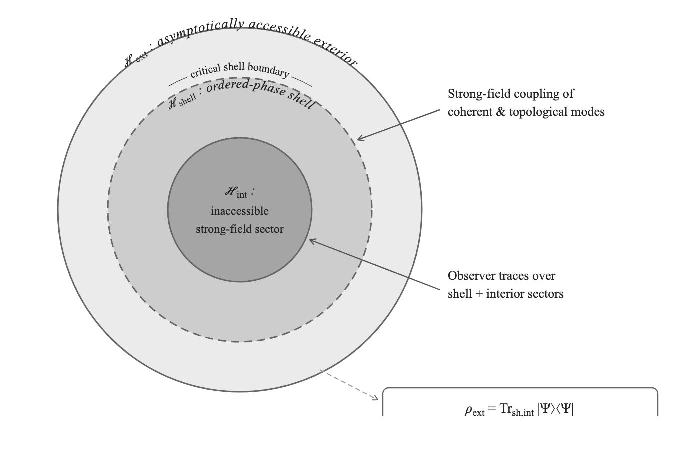
\includegraphics[width=0.85\textwidth]{fig_bh_shell.pdf}
\caption{The ECT picture of a black hole. The classical event horizon is replaced by a critical shell where the condensate amplitude reaches a critical value and the effective geometry transitions between regimes. Information is encoded in shell correlations. (\emph{Level~A for the no-information-loss argument; Level~B for the shell closure.})}
\label{fig:pop_bh}
\end{figure}

ECT reframes the black-hole horizon not as a fundamental singularity of causal structure but as an emergent interface in the condensate medium. This provides a microscopic language for why semiclassical Hawking thermality may survive while allowing controlled corrections. The present section organises the mechanism and its observable channels; it does not yet provide a complete first-principles microtheory of black holes.

If information falls into a black hole and the black hole evaporates via Hawking radiation, is the information lost? This is the information paradox --- one of the deepest problems in theoretical physics.

ECT addresses it at two levels (Fig.~\ref{fig:pop_bh}).

\textbf{Level~A (structural):} The total condensate state is never fundamentally mixed. In ECT, the apparent mixedness (thermal character) of Hawking radiation is a \emph{reduced-state} phenomenon: the external observer's density matrix $\rho_{\rm ext} = {\rm Tr}_{\rm shell,int}|\Psi\rangle\langle\Psi|$ is mixed because it traces over the shell and interior degrees of freedom, not because information has been destroyed. A conditional theorem establishes that exact thermality of the radiation is incompatible with unitary evaporation: if the condensate evolves unitarily (as posited), the radiation \emph{must} carry subtle correlations encoding the infalling information. This is a Level~A negative result: fundamental information loss is structurally forbidden.

\textbf{Level~B (shell closure):} The event horizon is replaced by a \textbf{critical shell} --- a surface where the condensate amplitude reaches a critical value and the effective ordered-phase geometry transitions between regimes. Shell entropy scales with area: $S = A/(4\ell_{\rm Pl}^2)$ (Bekenstein--Hawking formula, derived). A finite-memory shell model reproduces a Page-curve-like behaviour. These results are model-based (Level~B), not yet a full first-principles derivation of black-hole evaporation. The classical singularity at $r=0$ is replaced by a Euclidean core where the condensate transitions from the Lorentzian ordered phase back to the Euclidean disordered phase.


\section{The grandfather paradox}

ECT's emergent view of time dissolves the grandfather paradox structurally.

Classical causal paradoxes of time travel arise from trying to maintain two incompatible assumptions: that one can move backward along the physical time axis, and that causal chains remain linearly irreversible. The contradiction appears because the traveller is imagined as re-entering an already fixed causal sequence from within that sequence.

In the Euclidean picture, the coordinate $w$ is not a fundamental causal axis --- it is a spatial coordinate of the underlying substrate. Moving ``backward in $w$'' is not literal motion into an already-existing past; it is motion in the deeper Euclidean medium. The segment of $w$ that the agent leaves no longer contains that agent as an independent continuation, and worldlines can cross in the Euclidean picture without producing a contradiction of the classical type. Causal order belongs to the Lorentzian branch, where it emerges through the cone structure and where effectively irreversible macroscopic histories appear when $\Gamma_{\rm loop} \gg 1$.

The paradox is not ``solved'' by imposing a rule such as ``the universe forbids inconsistencies.'' It is dissolved by recognising that Lorentzian causal intuitions have a limited domain of validity: they apply within the emergent branch, not at the fundamental Euclidean level.

This is a conceptual statement about the ontology of time in ECT, not an operational claim that macroscopic backward time travel is physically available within the emergent Lorentzian branch.


\section{Analogue laboratory programme}

If ECT is correct, then superfluid liquids, Bose--Einstein condensates, and other condensed-matter systems are not merely ``analogies'' but realisations of the same condensate physics at a different scale: ordered medium $\to$ symmetry breaking $\to$ emergent Lorentzian kinematics $\to$ vacuum effects. Experiments in these systems are therefore tests of condensate vacuum physics at accessible scales. Key platforms include:

Superfluid $^4$He and Bose--Einstein condensates: phase-winding quantisation, vortex dynamics, Goldstone spectrum, and the condensate-mediated correlation structure.

Acoustic black holes (``dumb holes'') in BECs: analogue Hawking effect and critical-shell structure.

Condensate-reflecting boundary experiments: if a system can be designed whose boundaries genuinely reflect the soft condensate sector, it would test the boundary-sensitive vacuum response predicted by ECT. Standard metallic-plate Casimir experiments do not probe this channel.

Atom interferometry: gravitational decoherence channel predicted by ECT.


\section{Conclusions of Part~III}

\subsection{Principal results}

From the coherent branch, ECT derives or structurally motivates:

\begin{enumerate}
\item Hilbert-space structure via reflection positivity (\emph{A/B}).
\item Schr\"odinger and KG equations as descendants (\emph{A/B}).
\item Superposition, interference, Pauli exclusion (\emph{A/B}).
\item Quantisation from compact-phase winding (\emph{A}).
\item PES as organising principle (\emph{B}).
\item Born rule from RP inner product (\emph{B}).
\item Measurement through decoherence (\emph{A/B}).
\item Entanglement as common-medium correlation (\emph{A/B}).
\item Tunnelling as Euclidean passage (\emph{A/B}).
\item Casimir boundary-sensitive vacuum response (\emph{B, conditional}).
\item Unruh temperature (\emph{A/B}).
\item Gravitational decoherence channel (\emph{B}).
\item No fundamental information loss in BH (\emph{A}).
\item BH entropy $\propto$ area (\emph{B}).
\item Page curve from shell model (\emph{B}).
\item Quantum gravity dissolved by architecture (\emph{A/B}).
\end{enumerate}

\subsection{Key equations and principles of Part~III}

Winding condition: $\oint \partial_A\theta\,dX^A = 2\pi n$.

Elementary loop action: $S_{\rm loop,min} = 2\pi\hbar$.

PES: persistent configurations = extremal $\cap$ decoherence-resistant $\cap$ phase-compact.

Decoherence time: $\tau_{\rm dec} = 1/(N_{\rm eff}\gamma)$.

Casimir: boundary-sensitive vacuum response; provisional $3/2$ factor conditional on soft-mode counting and condensate-reflecting boundaries.

BH entropy: $S = A/(4\ell_{\rm Pl}^2)$.

\subsection{Part~III derivation logic}

\begin{figure}[H]
\centering

\includegraphics[width=\textwidth]{fig_partIII_derivation_logic_pop.pdf}
\caption{Part~III derivation logic. The coherent branch produces: Hilbert-space structure, wave equations, Born rule, decoherence, PES, vacuum effects, BH thermodynamics, and measurement theory. Colours indicate derivation levels.}
\label{fig:pop_partIII_logic}
\end{figure}

Figure~\ref{fig:pop_partIII_logic} shows the complete derivation architecture of Part~III.


\part{Summary, Comparisons, and Outlook}
\label{part:summary_pop}


\section{Architectural comparison with neighbouring programmes}

ECT is not the only attempt to address the foundational questions of physics. The following comparison locates it among its closest architectural neighbours.

\textbf{General Relativity + Standard Model:} Time and Lorentzian structure are fundamental. Gauge group is postulated. Quantum axioms are primitive. Dark sector requires extra particles + $\Lambda$. BH information paradox is open.

\textbf{Einstein--aether theory (Jacobson, 2004):} Lorentzian structure is fundamental; a preferred frame is added via a postulated unit vector $u^A$. In ECT, the orientation $n^A$ is derived from $\partial_A\Phi$, not postulated.

\textbf{Ho\v{r}ava--Lifshitz gravity:} Lorentz invariance is broken \emph{explicitly} at the fundamental level. In ECT, it is broken \emph{spontaneously} from a higher symmetry.

\textbf{Volovik's ``Universe in a Helium Droplet'':} Spacetime emerges from a condensate, but the analogy remains conceptual. ECT proposes that the condensate mechanism is the actual physical mechanism.

\textbf{Causal Dynamical Triangulations:} Lorentzian structure is imposed as a lattice constraint. ECT derives it from continuous SSB.

\textbf{Hartle--Hawking no-boundary proposal:} The Euclidean arena is a computational tool for defining path integrals. In ECT, it is the fundamental ontological entity.

\textbf{MOND (Milgrom, 1983):} The critical acceleration $g^\dagger$ is a universal free constant. In ECT, it is derived from condensate dynamics and is environment-dependent.

\textbf{Superfluid dark matter models:} Spacetime is pre-existing; a superfluid component is added as dark matter. In ECT, spacetime and the ``superfluid'' dynamics arise from the same condensate.

In all cases, ECT distinguishes itself by deriving structures that other theories postulate, and by unifying the dark, gravitational, and quantum sectors within a single condensate framework.


\section{Distinctive features of the framework}

Several features distinguish ECT from all other approaches:

\textbf{Single-field origin:} Everything --- spacetime, gravity, quantum mechanics, gauge interactions, dark sector phenomena --- emerges from one scalar field $\Phi$.

\textbf{No external time:} Time is derived from $O(4) \to O(3)$ SSB, not assumed. This is stricter than most quantum gravity approaches.

\textbf{``How'' and ``why'':} ECT reproduces quantum equations \emph{and} explains why they take the form they do (compact phase structure, reflection positivity, boundary-value vs.\ Cauchy problem).

\textbf{Honest epistemology:} Every result is classified as Level~A, B, or Open. No overclaiming.

\textbf{Cross-sector universality of $S_0$:} The same action scale controls phase weighting, wave kinematics, canonical normalisation, and Born weights simultaneously. This is falsifiable: if different quantum layers required different scales, ECT would be refuted.

\textbf{Unified dark sector:} Both ``dark matter'' and ``dark energy'' effects arise from condensate dynamics without new entities.

\textbf{Minimal parameter count:} The entire theory is controlled by four parameters: $\mu^2$, $\lambda$, $\alpha$, $\beta$. In the canonical benchmark $(\alpha, \beta) = (2, 1)$, only \textbf{two parameters} remain: $\mu^2$ and $\lambda$. From these two numbers, ECT derives $G_N$, $\hbar$, $c$, the entire equation hierarchy, the gauge structure, the gravitational sector, galaxy rotation curves, cosmological evolution, and the quantum formalism --- without introducing any additional free parameters, phenomenological fields, or ad hoc assumptions. No other current framework achieves comparable scope with comparable economy.


\section{Key equations, laws, and principles of ECT}

The following equations and principles define ECT not only qualitatively but in its applied, quantitative aspects:

\textbf{Foundational action:}
$S_E[\Phi] = \int d^4X\{\frac{1}{2}(\partial_A\Phi)^2 + V(\Phi)\}$, $V = -\frac{\mu^2}{2}\Phi^2 + \frac{\lambda}{4}\Phi^4$.

\textbf{Gradient condensate:}
$\langle\partial_A\Phi\rangle = u_0\,\delta_{Aw}$; breaks $O(4) \to O(3)$.

\textbf{Effective kinetic tensor:}
$K^{AB} = \beta\,\delta^{AB} - \alpha\,n^An^B$ (uniqueness theorem).

\textbf{Propagation speed:}
$c_* = \sqrt{\beta/(\alpha - \beta)}$ (= speed of light).

\textbf{Matching relations:}
$G_N = c_*^4/(8\pi\phi_0^2)$; \quad $\hbar = c_*\phi_0/\sqrt{\lambda}$.

\textbf{Cross-sector cone universality:}
$c_{\rm phase} = c_\gamma = c_{\rm GW} = c_*$.

\textbf{Loop quantisation:}
$\oint \partial_A\theta\,dX^A = 2\pi n$; \quad $S_{\rm loop,min} = 2\pi\hbar$.

\textbf{Second law:}
$dS_{\rm ent}/dw = N_{\rm eff}\gamma(dq/dw)^2 \geq 0$.

\textbf{Generalised Einstein equations:}
$G_{\mu\nu} + \Lambda_{\rm eff}g_{\mu\nu} = 8\pi G_{\rm eff}T_{\mu\nu} + \Theta_{\mu\nu}[n]$.

\textbf{Galactic interpolation:}
$g(R) = \frac{1}{2}(g_N + \sqrt{g_N^2 + 4g_Ng^\dagger})$.

\textbf{BTFR:}
$v_{\rm flat}^4 = G_N M_{\rm bar}\,g^\dagger$ (slope~4, algebraic).

\textbf{Hubble evolution:}
$G_{\rm eff}(z) \approx G_N(1+z)^{2\varepsilon}$, $\varepsilon \approx 0.01$.

\textbf{PES:}
Persistent configurations = extremal $\cap$ decoherence-resistant $\cap$ phase-compact.

\textbf{Decoherence time:}
$\tau_{\rm dec} = 1/(N_{\rm eff}\gamma)$.

\textbf{BH entropy:}
$S = A/(4\ell_{\rm Pl}^2)$.

\textbf{Casimir (conditional):}
$F_{\rm ECT} = \frac{3}{2}F_{\rm QED}$ in the provisional three-component
soft-orientation EFT with condensate-reflecting boundaries; not a
universal laboratory prediction.


\section{Falsifiable predictions}
\label{sec:pop_predictions}

Each prediction below is specific, quantitative, and testable:

\begin{enumerate}
\item \textbf{BTFR slope = 4} (\emph{A}). Algebraic consequence of the $\phi$-closure. A confirmed deviation would rule out the ECT galactic sector.

\item \textbf{$g^\dagger \propto cH_0$} (\emph{B}). Links galactic and cosmological scales. Testable by comparing $g^\dagger$ from galaxies with independently measured $H_0$.

\item \textbf{Fifth force: $\eta \sim 10^{-15}$} (\emph{B}). Within reach of MICROSCOPE-2 (current: $\eta < 10^{-14}$).

\item \textbf{Dark energy: $w_0 \approx -0.83$} (\emph{B}). Distinguishable from $w=-1$ by DESI/Euclid. Confirmed $w=-1$ falsifies ECT dark energy.

\item \textbf{Environmental modulation of $g^\dagger$} (\emph{B}). Field vs.\ cluster galaxies show different $g^\dagger$ --- absent in MOND.

\item \textbf{Casimir boundary-sensitive vacuum response} (\emph{B, conditional}). The ordered vacuum must respond to boundaries that reflect its soft sector. The provisional $3/2$ factor depends on naive Goldstone-coordinate counting and idealised condensate-reflecting boundaries; it is not a universal laboratory prediction for standard metallic plates.

\item \textbf{$M_{\rm max} = 2.17\,M_\odot$} (\emph{B}). Cf.\ PSR~J0740+6620 ($2.14\,M_\odot$). Pulsar with $M > 2.2\,M_\odot$ constrains this.

\item \textbf{CMB quadrupole deficit} (\emph{B/Open}). A structural argument for horizon-scale suppression exists, but the quantitative prediction of $\delta C_2/C_2$ remains open.

\item \textbf{No dark matter particles} (\emph{B}). Detection of a DM particle falsifies this prediction.

\item \textbf{$w \neq -1$} (\emph{B}). Dark energy is dynamical. Static $\Lambda$ at high precision rules out the mechanism.

\item \textbf{LIV: $\Delta t_{\rm GW} \sim 10^{-64}$\,s} (\emph{A/B}). Planck-suppressed. GW170817 bound satisfied.

\item \textbf{Proton stability} (\emph{C}). Conditional on the gauge/flavour completion: three selection-rule patterns are possible --- full low-energy protection (proton stable), partial protection ($\Delta B\!=\!1$ forbidden, $n$--$\bar n$ oscillations possible), or generic Planck-suppressed $\Delta B\!=\!1$ decay ($\tau_p \sim 10^{41}$--$10^{42}\,$yr). All consistent with Super-K limit $\tau_p > 2.4\times 10^{34}\,$yr. This is a Level~C closure discriminant, not a strict-core prediction.
\end{enumerate}

\section{Colour completion: a consistency requirement}
\label{sec:pop_colour}

The current ECT derivations impose a reverse-engineered constraint on the medium: any viable completion must contain an exact unbroken colour sector. A strict obstruction excludes colour-carrying condensates: any condensate transforming nontrivially under an internal group~$G$ breaks~$G$ to its stabilizer. Therefore the condensate must remain a colour singlet, and colour must reside in a separate internal sector.

The primary candidate completion assumes the medium carries a local complex rank-3 internal module with $SU(3)$-structure: a Hermitian metric and a distinguished antisymmetric trilinear form~$\varepsilon_{abc}$. Local non-rigidity of this module (extending the P5 logic) yields $SU(3)$ gauge redundancy. The preserved $\varepsilon_{abc}$ has a direct counterpart in observed physics: it is the tensor from which colour-neutral baryonic channels are constructed.

A deeper alternative is an internal $G_2$-structured fibre, where $SU(3)$ arises as the stabilizer of a unit internal direction: $\mathrm{Stab}_{G_2}(u) = SU(3)$. This would explain \emph{why} the colour group is exactly $SU(3)$, but requires exceptional internal geometry not otherwise forced by the postulates.

Neither completion yet derives full QCD: coupling~$g_s$, confinement, quark representations, and $\theta_{\rm QCD}$ remain open.

\begin{table}[H]
\centering
\small
\caption{Key status changes under the primary colour completion.}
\begin{tabular}{@{}p{3.2cm}p{3.2cm}p{3.2cm}p{3cm}@{}}
\toprule
Item & Before & After & Still open \\
\midrule
Colour symmetry & Missing & $SU(3)$ available & Dynamical realisation \\
Gauge bosons & 4 of 12 & $8+3+1=12$ at symmetry level & Full dynamics \\
Quark/lepton pattern & Inaccessible & Structurally compatible & Chirality, reps \\
Meson/baryon channels & Inaccessible & Singlet channels available & Bound-state dynamics \\
$\alpha_s$, $\Lambda_{\rm QCD}$ & Undefined & Definable targets & Not derived \\
Proton mass ($\sim\!938$\,MeV) & Inaccessible & Accessible in principle & Binding dynamics \\
$\alpha_{\rm fs}$ normalisation & Quark loops undefined & $Z_A$ strengthened & Full calculation open \\
Baryogenesis ($\eta_B$) & Baryon number incomplete & Colour defines baryon number & Transport open \\
Proton stability ($\tau_p$) & Selection rules not formulable & Three patterns (I/II/III) formulable & Pattern identification, channels open \\
\bottomrule
\end{tabular}
\end{table}


\section{Open problems}

These are stated explicitly as unsolved targets:

\begin{enumerate}
\item \textbf{Three fermion generations.} Qualitative routes exist (topological sectors of $S^3$); rigorous derivation of exactly three is not achieved.

\item \textbf{Yukawa hierarchy.} Mass differences from $m_e \sim 0.5$\,MeV to $m_t \sim 173$\,GeV not derived.

\item \textbf{$\alpha = 1/137$.} No first-principles prediction.

\item \textbf{Renormalisability.} Probable on fixed Euclidean background; not proven.

\item \textbf{Nonlinear GEE.} Structurally motivated (Level~B); full mathematical rigour not achieved.

\item \textbf{Born rule.} Motivated via RP inner product (Level~B); not a first-principles theorem.

\item \textbf{Bell correlators.} Medium-based entanglement established; explicit correlators not derived.

\item \textbf{BH evaporation.} Page curve from toy model (Level~B); full dynamics open.

\item \textbf{High-$z$ background.} Self-consistent $\phi_b(z)$ at $z \gg 1$ not derived.

\item \textbf{Gradient condensation (OP-grad).} Dynamical origin of ordered branch from bare P3: the deepest open problem.

\item \textbf{Graviton-loop power counting (OP-UV1).} Explicit one-loop graviton power counting in the ECT condensate background. Structurally expected to be tame (Landau pole far above EFT threshold), but not yet computed.

\item \textbf{Two-loop RG of the condensate--graviton system (OP-UV3).} Full RG flow including condensate--graviton mixing; needed to establish the UV behaviour beyond the scalar closure.

\item \textbf{OS reconstruction for spin-2 sector (OP-OS1).} Reflection positivity for the orientation (tensor) sector. If established, graviton states appear automatically in the Hilbert space without a separate quantisation act.

\item \textbf{Cosmological-constant fine-tuning (OP-$\Lambda$3).} The tree-level condensate minimum gives $V(\phi_0)=-\mu^4/(4\lambda)$, a large negative contribution. ECT reframes (finite loop corrections, dynamical $\Lambda_{\rm eff}$) but does not yet eliminate the residual fine-tuning of $\sim 10^{-120}$.

\item \textbf{Proton stability and baryon-number selection rules (OP-proton).} Derivation of which baryon-number selection-rule pattern (full protection / partial $\Delta B\!=\!2$ only / generic $\Delta B\!=\!1$) is realised in the completed gauge/flavour sector; if generic violation, identification of decay channels and coefficient structure.
\end{enumerate}

\section{Complete derivation map}

\begin{figure}[H]
\centering

\includegraphics[width=\textwidth]{fig_ect_derivation_map_pop.png}
\caption{Complete ECT derivation map. The full logical architecture from the $\Phi$-medium and the six postulates through all four Parts of the theory. Colours indicate postulates (dark), phenomenological inputs (grey), Level~A (light grey), Level~B (white), and Open (dashed).}
\label{fig:pop_fullmap}
\end{figure}

Figure~\ref{fig:pop_fullmap} shows the complete derivation architecture of ECT.


\section{Open problems of physics addressed within ECT}

Within its framework, ECT addresses several well-known open problems of modern physics:

\begin{enumerate}
\item \textbf{Unification of quantum mechanics and gravity.} Both emerge from the same ordered condensate. The unification is architectural, not forced (\emph{A/B}).

\item \textbf{The origin of time.} Why does spacetime have signature $(-,+,+,+)$? Derived from $O(4)\to O(3)$ SSB (\emph{A}).

\item \textbf{The dark matter problem.} No DM particle has been detected despite decades of searches. ECT reinterprets all observational phenomena as condensate dynamics; the minimal benchmark does not require DM particles (\emph{B}).

\item \textbf{The cosmological constant problem.} QFT predicts $\Lambda$ that is $10^{120}\times$ too large. ECT replaces $\Lambda$ with dynamical condensate energy, naturally small (\emph{B}).

\item \textbf{The Hubble tension.} $>5\sigma$ discrepancy. ECT provides structural alleviation through evolving $G_{\rm eff}$ (\emph{sign: A; magnitude: B}).

\item \textbf{JWST early galaxies.} Enhanced early gravity + $\Theta_{\mu\nu}$ accelerate structure formation (\emph{B}).

\item \textbf{Baryon asymmetry.} Native leptogenesis: $\eta_B \sim 9\times10^{-10}$ vs.\ observed $6\times10^{-10}$ (\emph{A/B}).

\item \textbf{Black-hole information paradox.} Fundamental information loss structurally forbidden (\emph{A}); Page curve reproduced (\emph{B}).

\item \textbf{The measurement problem.} Explained through decoherence, no collapse postulate (\emph{A/B}).

\item \textbf{The origin of quantum mechanics.} Hilbert space, superposition, Born rule derived from condensate (\emph{A/B}).

\item \textbf{The arrow of time.} Derived from condensate ordering and decoherence monotonicity (\emph{A/B}).

\item \textbf{The need for inflation.} Four cosmological problems resolved without inflaton, avoiding inflation's paradoxes (\emph{A/B}).

\item \textbf{The hierarchy problem.} $M_{\rm Pl}/M_{\rm EW} \sim 10^{16}$ addressed through running coupling (\emph{B/Open}).

\item \textbf{Why $3+1$ dimensions?} The $O(4)\to O(3)$ transition singles out exactly three spatial directions and one temporal seed. Standard physics postulates $d=3+1$ without explanation (\emph{A}).

\item \textbf{Why no magnetic monopoles?} $\pi_2(S^3)=0$: topological anti-prediction. GUT frameworks generically predict monopoles; ECT excludes them (\emph{A}).

\item \textbf{Vacuum stability.} The ordered condensate has $V''(\phi_0)>0$. In the Standard Model, the electroweak vacuum is metastable at $m_h=125$\,GeV (\emph{A}).

\item \textbf{Quantum gravity.} No need to quantise geometry: gravity is a condensate response, the graviton a condensate excitation on a fixed Euclidean background (\emph{A/B}).

\item \textbf{Cosmological coincidence question.} The ``why now'' question --- why $\Omega_m$ and $\Omega_\Lambda$ are of comparable order today --- is debated in the literature, since in pure $\Lambda$CDM the order-unity window of $\rho_m/\rho_\Lambda$ already spans a sizeable low-redshift range, and its force depends on measure and observer-selection assumptions. In ECT dark energy is supplied by the slow-rolling amplitude of the same ordered condensate that generates $G_N$, $c_*$ and $\hbar$, which makes the question structurally well-posed rather than built in by hand. In the current calibrated thawing benchmark, however, the condensate dark-energy density varies by only ${\approx}11\%$ across the observable redshift range, and the corresponding order-unity window in $\rho_m/\rho_\phi$ is only marginally wider than in pure $\Lambda$CDM. We therefore do not list coincidence alleviation among current ECT results; it remains an open programmatic question, distinct from the separate $10^{-120}$ vacuum-scale fine-tuning (\emph{Level~B/C-Open}).

\item \textbf{Massless graviton.} The spin-2 mode emerges from SSB with $m_g=0$ protected by gauge structure, consistent with the LIGO bound $m_g<1.2\times10^{-22}$~eV (\emph{A/B}).
\end{enumerate}

The breadth of problems addressed from a single starting point is a distinctive feature of the framework.


\section{Conclusion}

ECT is an attempt to place spacetime, gravity, and quantum behaviour within a single pre-spacetime framework. In its current form, some parts of this programme are structural results, some are closure-dependent effective constructions, and some remain open.

\textbf{What is established structurally (Level~A):}
Lorentzian signature from $O(4) \to O(3)$ SSB; universal causal cone ($c_* = c$); the equation hierarchy (Euclidean $\to$ KG $\to$ Schr\"odinger); arrow of time from retarded decoherence; BTFR slope exactly~4; resolution of the horizon, flatness, and monopole problems; structural impossibility of fundamental information loss in black holes.

\textbf{What is obtained at effective/closure level (Level~B):}
Newton's constant, Planck's constant, and $c$ as condensate matching relations; generalised Einstein equations with $\Theta_{\mu\nu}$; dark energy as condensate residual energy ($w_0 \approx -0.83$); Hubble tension alleviation ($\Delta H_0 \sim +3$\,km/s/Mpc); galaxy rotation curves for 165 SPARC galaxies ($\chi^2/N \approx 2.95$); reinterpretation of the dark sector as condensate dynamics; decoherence and the quantum--classical boundary; BH area entropy and Page-curve-like behaviour from the shell model; PES; boundary-sensitive Casimir vacuum response (conditional).

\textbf{What remains an open programme:}
Three fermion generations; Yukawa hierarchy; $\alpha = 1/137$; renormalisability; Born rule as first-principles theorem; Bell correlators; complete BH evaporation; gradient condensation from bare P3; proton stability as a UV discriminant (three selection-rule patterns conditional on gauge/flavour completion).

\textbf{Distinctive conceptual achievements (not available in standard physics):}
The effective metric is derived, not fundamental---the condensate is primary, geometry is secondary.
Three logically distinct classes of excitations replace the uniform field-postulate structure of QFT.
The axioms of QM are relocated from postulates to reconstruction targets.
Event-like interaction is emergent; in the coherent branch, subsystems are related by common-medium correlation.
Gravitational decoherence is derived without the Di\'osi--Penrose postulate (nanosphere prediction: $\tau\sim 38$\,ms).
A recoherence law $P_{\rm back}/P_{\rm fwd}=e^{-\Gamma_{\rm loop}}$ is predicted; standard QM has no analogue.
Fock space is a reconstruction target, not a foundational axiom.

\begin{table}[H]
\centering
\caption{Distinctive ECT outputs and foundational questions addressed.}
\label{tab:pop_distinctive}
\small
\renewcommand{\arraystretch}{1.15}
\begin{tabular}{@{}p{3.8cm}p{4.5cm}cp{2.2cm}@{}}
\toprule
Problem / Achievement & ECT mechanism & Level & Unique? \\
\midrule
\multicolumn{4}{l}{\textit{Conceptual achievements}} \\
\midrule
Metric derived & Condensate primary, geometry secondary & A/B & Yes \\
Three particle classes & Required / embedded / topological & A/B & Yes \\
QM axioms $\to$ targets & Reconstructed, not postulated & A/B & Yes \\
Interaction = Lorentzian & Coherent branch: correlation only & A & Yes \\
Fock as reconstruction target & Variable $N$ = condensate reconfiguration & Open & Yes (conceptual) \\
\midrule
\multicolumn{4}{l}{\textit{Foundational questions}} \\
\midrule
Why $3\!+\!1$ dimensions? & $O(4)\!\to\!O(3)$ & A & Yes \\
No monopoles & $\pi_2(S^3)\!=\!0$ & A & Anti-prediction \\
Vacuum stability & $V''(\phi_0)\!>\!0$ & A & Yes \\
Quantum gravity & No metric quantisation & A/B & Architecture \\
Massless graviton & Spin-2 from ordered branch, gauge-protected & A/B & Structural \\
\midrule
\multicolumn{4}{l}{\textit{Quantitative predictions}} \\
\midrule
Grav.\ decoherence & $\tau\!\sim\!38$\,ms (nanosph.) & B & No DP postulate \\
Recoherence law & $P_{\rm back}/P_{\rm fwd}\!=\!e^{-\Gamma}$ & B & Yes \\
$w_0\!\approx\!-0.83$ & Condensate residual & B & DESI/Euclid \\
5th force $\eta\!\sim\!10^{-15}$ & Fermion--condensate & B & MICROSCOPE-2 \\
\bottomrule
\end{tabular}
\end{table}

In its minimal closure, ECT does not require dark-matter particles, a fundamental cosmological constant, an inflaton field, separate quantum axioms, or an ad hoc collapse postulate as independent starting ingredients. With at most four bare parameters --- reducible to two in the canonical benchmark --- ECT addresses a scope that typically requires many independent inputs in the standard framework.

Whether ECT ultimately becomes a viable theory of nature or remains a productive conceptual laboratory, it does something valuable: it demonstrates that spacetime, gravity, and quantum mechanics \emph{can} be derived from a common substrate, and it identifies the specific structures --- gradient condensation, compact-phase topology, orientation stiffness, and the Principle of Euclidean Stationarity --- that make this possible.

If even partly correct, the deepest truth about reality is not that the universe \emph{contains} time, but that under the right conditions, the universe \emph{creates} it.

\vspace{2em}
\noindent\rule{\textwidth}{0.5pt}

\noindent\textbf{Note.}
This article is a narrative companion to:
\emph{``Euclidean Condensate Theory (ECT): Emergence of Spacetime,
Quantum Mechanics, and Gravity from Spontaneous $O(4)$ Symmetry
Breaking''} by Valeriy Blagovidov (2026).
Full preprint: \href{https://doi.org/10.5281/zenodo.18917929}{doi:10.5281/zenodo.18917929}.

\medskip
\centerline{\url{https://github.com/chufelo/ECT-preprint-code}}
\medskip
\centerline{Zenodo: \url{https://doi.org/10.5281/zenodo.18917929}}

\end{document}
